\chapter{Modelaci\'on de dependencias mediante la teor\'ia de c\'opulas.}
\label{ch:copulaTheory}

La metodolog\'{i}a moderna para modelar dependencias estoc\'{a}sticas es la teor\'ia de c\'opulas. \'Esta ha demostrado m\'{a}s generalidad y versatilidad que el enfoque de regresi\'{o}n cl\'{a}sico (lineal, por ejemplo) para modelar dependencias.

Aunque la teor\'ia de c\'opulas no es una teor\'ia tan nueva \citep{sklar_fonctions_1959}, se han dado pocas aplicaciones pr\'acticas. Dentro de la industria petrolera se han hecho algunas aplicaciones para simular conjuntamente propiedades petrof\'isicas usando c\'opulas \citep{diaz-viera_stochastic_2006,diaz-viera_spatial_2012,diaz-viera_stochastic_2006-2,diaz-viera_stochastic_2005-1,diaz-viera_stochastic_2005,erdely_modeling_2011,erdely_joint_2012,erdely_trivariate_2012,erdely_nonparametric_2009,hernandez-maldonado_simulacion_2014,hernandez-maldonado_joint_2012,hernandez-maldonado_joint_2012-1,hernandez-maldonado_trivariate_2012} pero a\'un no se han hechos trabajos respecto a las propiedades de fractura.

Desde un punto de vista, las c\'opulas son funciones que unen o ``acoplan'' funciones de distribuci\'on multivariada a sus funciones de distribuci\'on marginal unidimensional. No existen modelos cl\'asicos que combinen de manera general datos orientados con datos no orientados por lo que con este trabajo se propondr\'an modelos que de manera adecuada tomen en cuenta la dependencia con la c\'opula, y a la vez respeten y reproduzcan las marginales.

\section{Generalidades}

?`Qu\'e relaci\'on existe entre una funci\'on de distribuci\'on multivariada, \(H\), y sus funciones de distribuci\'on marginal, \(F\) y \(G\)? La soluci\'on a este problema la dio \cite{sklar_fonctions_1959} al crear una nueva clase de funciones a las que llam\'o c\'opulas.

Para poder abordar adecuadamente la definici\'on de c\'opulas y el teorema de \cite{sklar_fonctions_1959} observemos primero algunas definiciones.

Sean \({S_{1},S}_{2} \subset \overset{\overline{}}{\mathbb{R}}\) y \(H:S_{1} \times S_{2}\mathbb{\rightarrow R}\). Si denotamos al \'infimo como ``\(\mathrm{\inf}\)'', y suponemos que \({a_{1} = \mathrm{\text{inf\ }}S}_{1}\), \(a_{2} = \mathrm{\inf}\ S_{2}\), decimos que \(H\) est\'a \emph{aterrizada} si \(H\left( x,a_{2} \right) = 0 = H\left( a_{1},y \right)\) para todo \(\left( x,y \right) \in S_{1} \times S_{2}\).De igual manera, si denotamos al supremo como ``\(\mathrm{\sup}\)'', y suponemos que \({b_{1} = \mathrm{\text{sup\ \ }}S}_{1}\) y \(b_{2} = \mathrm{\sup}\ S_{2}\), decimos que una funci\'on \(H\) tiene \emph{marginales}, y que las marginales de \(H\) son las funciones \(F\) y \(G\) dadas por

\(\mathrm{\text{Dom}}\ F = S_{1}\) y \(F\left( x \right) = H\left( x,b_{2} \right)\) para todo \(x \in S_{1}\)

\(\mathrm{\text{Dom}}\ G = S_{2}\) y
\(G\left( x \right) = H\left( b_{2},y \right)\) para todo
\(y \in S_{2}\)

\noindent
Donde ``\(\mathrm{\text{Dom}}\)'' denota el dominio de la funci\'on
correspondiente.

Sean \({S_{1},S}_{2} \subset \overset{\overline{}}{\mathbb{R}}\), y
\(B = \left\lbrack x_{1},y_{1} \right\rbrack \times \left\lbrack x_{2},y_{2} \right\rbrack\)
un rect\'angulo tal que todos sus v\'ertices est\'an en \(S_{1} \times S_{2}\). Una funci\'on \(H:S_{1} \times S_{2}\mathbb{\rightarrow R}\) es bi-creciente si,

\begin{equation}
    \Delta_{xy}H(x,y) := \Delta_{x} \left(\Delta_{y}H(x,y)\right)
    = H(x_2,y_2) - H(x_2,y_1) - H(x_1, y_2) + H(x_1, y_1) \ge 0
	\label{eq:monotoneContstraint2D}
\end{equation}

\textbf{Definici\'on. Subc\'opula.} Una subc\'opula bidimensional (o 2-subc\'opula) es una funci\'on \(C'\) con las siguientes caracter\'isticas:

\begin{enumerate}
\item
  \(\mathrm{\text{Dom}}C^{'} = S_{1} \times S_{2}\) donde \(S_{1}\) y
  \(S_{2}\) son subconjuntos de  \(\mathbb{I =}\left\lbrack 0,1 \right\rbrack\) que contienen al cero y a 1,
\item
  \(C'\) est\'a aterrizada y es bi-creciente.
\item
  Para cada \(u \in S_{1}\), \(C^{'}\left( u,1 \right) = u\); y para
  cada \(v \in S_{2}\), \(C^{'}\left( 1,v \right) = v\).
\end{enumerate}

\textbf{Definici\'on. C\'opula.} Una c\'opula bidimensional (\'o 2-c\'opula) es una 2-subc\'opula \(C\) tal que \(\mathrm{\text{Dom}}\ C = \mathbb{I}^{2}\).

\textbf{Teorema de \cite{sklar_fonctions_1959}.} Sea \(H\) una funci\'on de distribuci\'on con funciones marginales \(F\) y \(G\). Entonces existe una c\'opula \(C\) tal que para todo \(x,y \in \overset{\overline{}}{\mathbb{R}}\),

\begin{equation}
	H(x,y) = C(F(x),G(y))
	\label{eq:sklarTheorem}
\end{equation}

Si \(F\) y \(G\) son continuas, entonces \(C\) es \'unica, de otra manera \(C\) est\'a determinada de manera \'unica en \(\mathrm{\text{Ran}}\ F \times \mathrm{\text{Ran}}\text{\ G}\). Si \(C\) es una c\'opula y \(F\) y \(G\) son funciones de distribuci\'on, entonces la funci\'on \(H\) definida por la ecuaci\'on \autoref{eq:sklarTheorem} es una funci\'on de distribuci\'on conjunta con marginales \(F\) y \(G\).

En la teor\'ia cl\'asica de c\'opulas se suponen modelos param\'etricos tanto para \(H\) como para las marginales \(F\) y \(G\). Por ejemplo, \(F\) pudiera ser \textit{normal} con par\'ametros \(\mu\) y \(\sigma^{2}\); y \(G\) \textit{exponencial} con par\'ametro \(\lambda\), mientras \(H\) la distribuci\'on normal bivariada con sus correspondientes par\'ametros.

Los modelos param\'etricos son importantes en varios aspectos.
Por ejemplo, sus par\'ametros proveen una interpretaci\'on r\'apida del fen\'omeno en estudio.
Existen todo un cat\'alogo de modelos \citep{nadarajah_compendium_2016} que explican una gran variedad de fen\'omenos.
Cuando se tiene poca confianza en los datos \'o se cuenta con modelos hipot\'eticos, se pueden probar ciertos modelos param\'etricos.
Generalmente, son m\'as f\'aciles de implementar computacionalmente que los modelos no param\'etricos y m\'as r\'apidos.

Como complemento a los modelos param\'etricos se tienen los modelos no-param\'etricos. Estos \'ultimos son realmente \'utiles cuando la estructura de dependencia es m\'as compleja que relaciones mon\'otonas entre variables \'unicamente \citep{joe_dependence_2014}. En el caso de existir marginales con formas complicadas (no sim\'etricas, multimodales, etc.), entonces el enfoque param\'etrico puede ser aplicado a la distribuci\'on multivariada directamente.

El ejemplo m\'as simple de una c\'opula no param\'etrica es la c\'opula emp\'irica, que se puede definir de la siguiente manera \citep{deheuvels_fonction_1979,fermanian_weak_2004,berghaus_weak_2017,radulovic_weak_2017,bucher_empirical_2011,carnicero_non-parametric_2013}.
Dada una muestra \(\left\{ \left( x_{1},y_{1} \right),\ \ldots,\ \left( x_{n},y_{n} \right) \right\}\) de la funci\'on de distribuci\'on conjunta del vector aleatorio \(\left( X,Y \right)\); con sus correspondientes pseudo-observaciones obtenidas mediante la \autoref{e:empF}.
Entonces, la funci\'on de distribuci\'on c\'opula emp\'irica se define como,

\begin{equation}
	{\hat{C}}_{n}\left( u,v \right) = \frac{1}{n}\sum_{i = 1}^{n}{\mathbbm{1}(u_{i} \leq u,v_{i} \leq v)}
	\label{e:empCopC} % 'emp'irical 'cop'ula 'c'ontinous case
\end{equation}

\noindent
Para \(1 \leq i \leq n\) donde
\(\mathbbm{1}(a \leq b,c \leq d)\) si \(a \leq b\) y \(c \leq d\) y cero en otro caso, con \(a,b,c,d\mathbb{\in R}\).

La \autoref{e:empCopC} se puede reescribir de la forma de la \autoref{e:empCopI}:

\begin{equation}
	n\hat{C}_{n}( u,v) =
	\sum_{i = 1}^{n}
	\mathbbm{1}(u_{i} \leq u,v_{i} \leq v)
	\label{e:empCopI} % 'emp'irical 'cop'ula 'I'nteger case
\end{equation}

De esta manera $n\hat{C}_n$, de manera an\'aloga a la forma emp\'irica univariada (\autoref{e:empF}), puede ser almacenado como un arreglo bidimensional de enteros sin signo.
Esto conlleva a evitar errores de redondeo que se puedan propagar ya que, para $n$ grandes, digamos $n=1\e{6}$, lo normal en estos tiempos, $1/n=1\e{-6}=0.000001$.
Adem\'as, tambi\'en hay un ahorro considerable en la memoria de la computadora. Como ventaja adicional, ayuda a obtener visualizaciones m\'as sencillas del algoritmo num\'erico para almacenar los valores de la c\'opula emp\'irica.

Para encontrar cualquier valor $\hat{C}_n(u,v)$ simplemente se compara $(u,v)$ con los valores $(u_i, v_i)$ siguiendo la funci\'on indicador y de forma acumulativa 2-creciente (hacia la derecha y hacia la arriba).

\begin{figure}
	\centering
	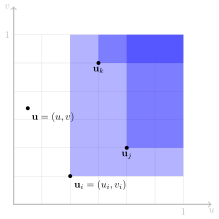
\includegraphics{empCopExplained}
	\caption{Donde $i,j,k \in \{1, \ldots,n\}$. Tonos m\'as oscuros representan valores de $n\hat{C}_n$ m\'as grandes. Cada cambio en tono representa una diferencia de uno (por la funci\'on indicador).}
	\label{f:empCopExplained}
\end{figure}

Esta forma permite un diagrama m\'as sencillo que relaciona la ubicaci\'on en el gr\'afico de pseudo-observaciones con su correspondiente arreglo en memoria de la computadora.
Supongamos que los datos $\{(x_i, y_i)\}$ est\'an ordenados por valores de $x$ crecientes, es decir, $u_i = u_{(i)}$. Esto no implica que $v_i = v_{(i)}$.
Adem\'as, suponemos que no hay valores repetidos.

\begin{figure}
	\centering
	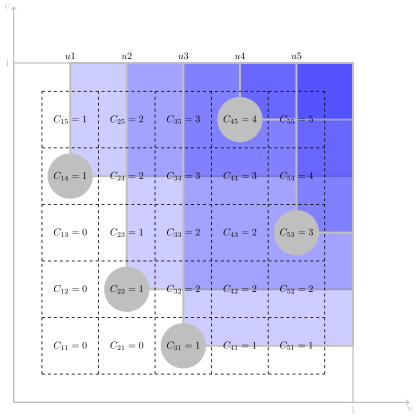
\includegraphics{empCopArray}
	\caption{Representaci\'on gr\'afica de la c\'opula emp\'irica y su relaci\'on con su almacenaje computacional en una matriz. El centro de cada c\'irculo representa una pseudo-observaci\'on $\mathbf{u}_i = (u_i,v_i)$. La malla regular de l\'ineas de guiones representa el arreglo en la memoria, $n\mathbf{C}$, que guarda los valores enteros $C_{ij}:=n\hat{C}_n(u_i, v_j)$. Donde $i$ denota el rengl\'on y $j$ la columna.
N\'otese que las $u_i$ est\'an ordenadas crecientemente pero no existe un orden en las $v_i$. Alternativamente se pudo haber ordenado por $v_i$ y dejar las $u_i$ sin orden.}
	\label{f:empCopArray}
\end{figure}

Para ligar la \autoref{f:empCopArray} con su correspondiente representaci\'on matricial $n\mathbf{C}$ (\autoref{e:empCopArray}), se referir\'a a la primera mediante palabras como horizontal/vertical, o paralelo al eje $u$/$v$; mientras que para referirse al correspondiente arreglo/matriz computacional se nombrar\'an renglones y columnas. Por ejemplo, el segundo rengl\'on de la matriz $n\mathbf{C}$, $n\mathbf{C}(2,\cdot)$, corresponde al rect\'angulo vertical de la \autoref{f:empCopArray} centrado en $u_2$, paralelo al eje $v$.

\begin{equation}
	n\mathbf{C} =
		\begin{pmatrix}
			C_{11} & C_{12} & C_{13} & C_{14} & C_{15}\\
			C_{21} & C_{22} & C_{23} & C_{24} & C_{25}\\
			C_{31} & C_{32} & C_{33} & C_{34} & C_{35}\\
			C_{41} & C_{42} & C_{43} & C_{44} & C_{45}\\
			C_{51} & C_{52} & C_{53} & C_{54} & C_{55}\\
		\end{pmatrix}
		=
		\begin{pmatrix}
			0 & 0 & 0 & 1 & 1\\
			0 & 1 & 1 & 2 & 2\\
			1 & 2 & 2 & 3 & 3\\
			1 & 2 & 2 & 3 & 4\\
			1 & 2 & 3 & 4 & 5
		\end{pmatrix}
	\label{e:empCopArray}
\end{equation}

Veamos el arreglo en la \autoref{f:empCopArray} por columnas, es decir, por rect\'angulos verticales de ancho $\Delta u_i$ y centrados en cada una de las pseudo-observaciones. 
N\'otese que, si fijamos un rengl\'on, digamos el rengl\'on $k$ que corresponde a $u_k$, los valores de $n\mathbf{C}$ satisfacen la siguiente relaci\'on de recurrencia:

\begin{equation}
	n\mathbf{C}(k,   ) =
	n\mathbf{C}(k-1, ) + \mathbf{v}_k
	\label{e:empCopRR}
\end{equation}

\noindent
donde el vector $\mathbf{v}_k := (0,0,\ldots,0,1,1,\ldots,1)$ contiene su primer $1$ en la entrada $rank(v_k)$, el rango de $v_k$.
Si $n \mathbf{C}$ fue inicializada con puros $0$, entonces se puede ahorrar memoria omitiendo la creaci\'on de un nuevo arreglo $\mathbf{v}_k$ al utilizar $n \mathbf{C}(k, ) := \mathbf{v}_n$.
Alternativamente, se puede proceder, primero por columnas y luego por renglones para obtener el mismo resultado.
La preferencia depender\'a del paradigma del arreglo en memoria del lenguaje de programaci\'on utilizado: \textit{row major} \'o \textit{column major}.
Tambi\'en se puede hacer m\'as eficiente al observar que el \'ultimo rengl\'on y la \'ultima columna tienen entradas correspondientes a $1,2,3,4,5$, para este caso. En el caso general tendr\'an entradas $1,2,\ldots,n$.
La implementaci\'on computacional de esta matriz se encuentra en la funci\'on \verb|bernsteincop::empCopM|, La funci\'on \verb|bernsteincop::genmat.copem| implementa un algoritmo similar pero no igual ya que compara los valores de $v_i$ en lugar de tomar el rango.

Para calcular el valor de la c\'opula emp\'irica en cualquier posici\'on $(u,v)$ solamente basta con saber los m\'aximos \'indices $i$ y $j$ que cumplen $(u_i,v_j) \le (u,v)$ elemento-a-elemento. Y $ \hat{C}_n(u,v) = n\mathbf{C}(i,j) / n$ (ver la \autoref{f:empCopExplained}).

N\'otese que la \autoref{e:empCopC} se puede escribir de la siguiente forma m\'as compacta y m\'as parecida a su contraparte univariada (\autoref{e:empF}):

\begin{equation}
	\hat{C}_{n}(\mathbf{u}) =
	\frac{1}{n} \sum_{i = 1}^{n}
	\mathbbm{1} (\mathbf{u}_{i} \leq \mathbf{u})
	\label{e:empCopV} % 'emp'irical 'cop'ula 'V'ectorized form
\end{equation}

\noindent
donde $\mathbf{u}_i := (u_i, v_i)$, $\mathbf{u}:=(u,v)$ y la relaci\'on de orden, $\le$, se efect\'ua componente a componente.


%Las c\'{o}pulas $C$ son funciones multivariadas, con ciertas caracter\'{i}sticas \citep[ch. 2]{nelsen_introduction_2006}, y que acoplan funciones de distribuci\'{o}n conjuntas $H$ y sus marginales univariadas $F_i$ de la siguiente manera para el caso bivariado \citep{sklar_fonctions_1959}:

%\begin{equation}
%\label{e:sklarT} % "e"quation of" Sklar" 's "T"heorem
%H(x_1,x_2)=C(F_1(x_1),F_2(x_2))
%\end{equation}

%De esta manera, la estructura de dependencia --capturada en la c\'{o}pula-- se puede modelar sin importar las funciones marginales univariadas.

Se puede ver que la c\'opula emp\'irica no es continua. Un modelo continuo de estructura de dependencia asociada dos variables aleatorias continuas e independientes $X$ y $Y$ es:

\begin{equation}
C_{XY}(u,v) = \Pi (u, v) := uv
\label{e:IndCop}
\end{equation}

Aunque la c\'opula emp\'irica no es continua, ella es \'util para obtener versiones continuas de la c\'opula.

\section{C\'opulas bivariadas de Bernstein}

Una versi\'on continua de la c\'opula emp\'irica se puede obtener mediante un ajuste polinomial. Una base del espacio de polinomios de grado $n$ son los polinomios de Bernstein (v\'ease la \autoref{s:bezier1D}):

\begin{equation}
	B(w|k,n):=\binom{k}{n} w^k (1 - w)^{n-k}
	\label{eq:bernsBasis}
\end{equation}

\noindent
donde $w \in [0,1]$, $k \in \{0,1, \ldots, n\}$.

Muchos lenguajes de programaci\'on tienen implementada eficientemente esta funci\'on, conocida en estad\'istica como la funci\'on de masa binomial. Por ejemplo, en \verb|R| est\'a implementada bajo el nombre \verb|dbinom|. Estos polinomios pueden ser utilizados para aproximar y suavizar la c\'opula emp\'irica (\autoref{e:empCopC}), lo que nos lleva a la c\'opula emp\'irica de Bernstein propuesta por \cite{sancetta_bernstein_2004}:

\begin{equation}
	C_B(u,v)=\sum_{i=0}^n \sum_{j=0}^n
	\hat{C}_n 
	\left(
	\frac{i}{n},\frac{j}{n}
\right)
B(u|i,n) B(v|j,n)
\end{equation}

En esta definici\'on, la c\'opula emp\'irica est\'a definida incluso para valores $u=0$, mientras que en la definici\'on de la funci\'on acumulativa emp\'irica (\autoref{e:empF}) la m\'inima pseudo-observaci\'on tomaba el valor $u_1 = 1/n$. Este inconveniente se resuelve a\~nadiendo $u_0 = 0$ \citep{sancetta_bernstein_2004} al vector de pseudo-observaciones emp\'iricas. Un ejemplo de la aplicaci\'on de esta teor\'ia en ciencias de la Tierra se muestra en la \autoref{f:phiK}.

\begin{figure}[H]
	\centering
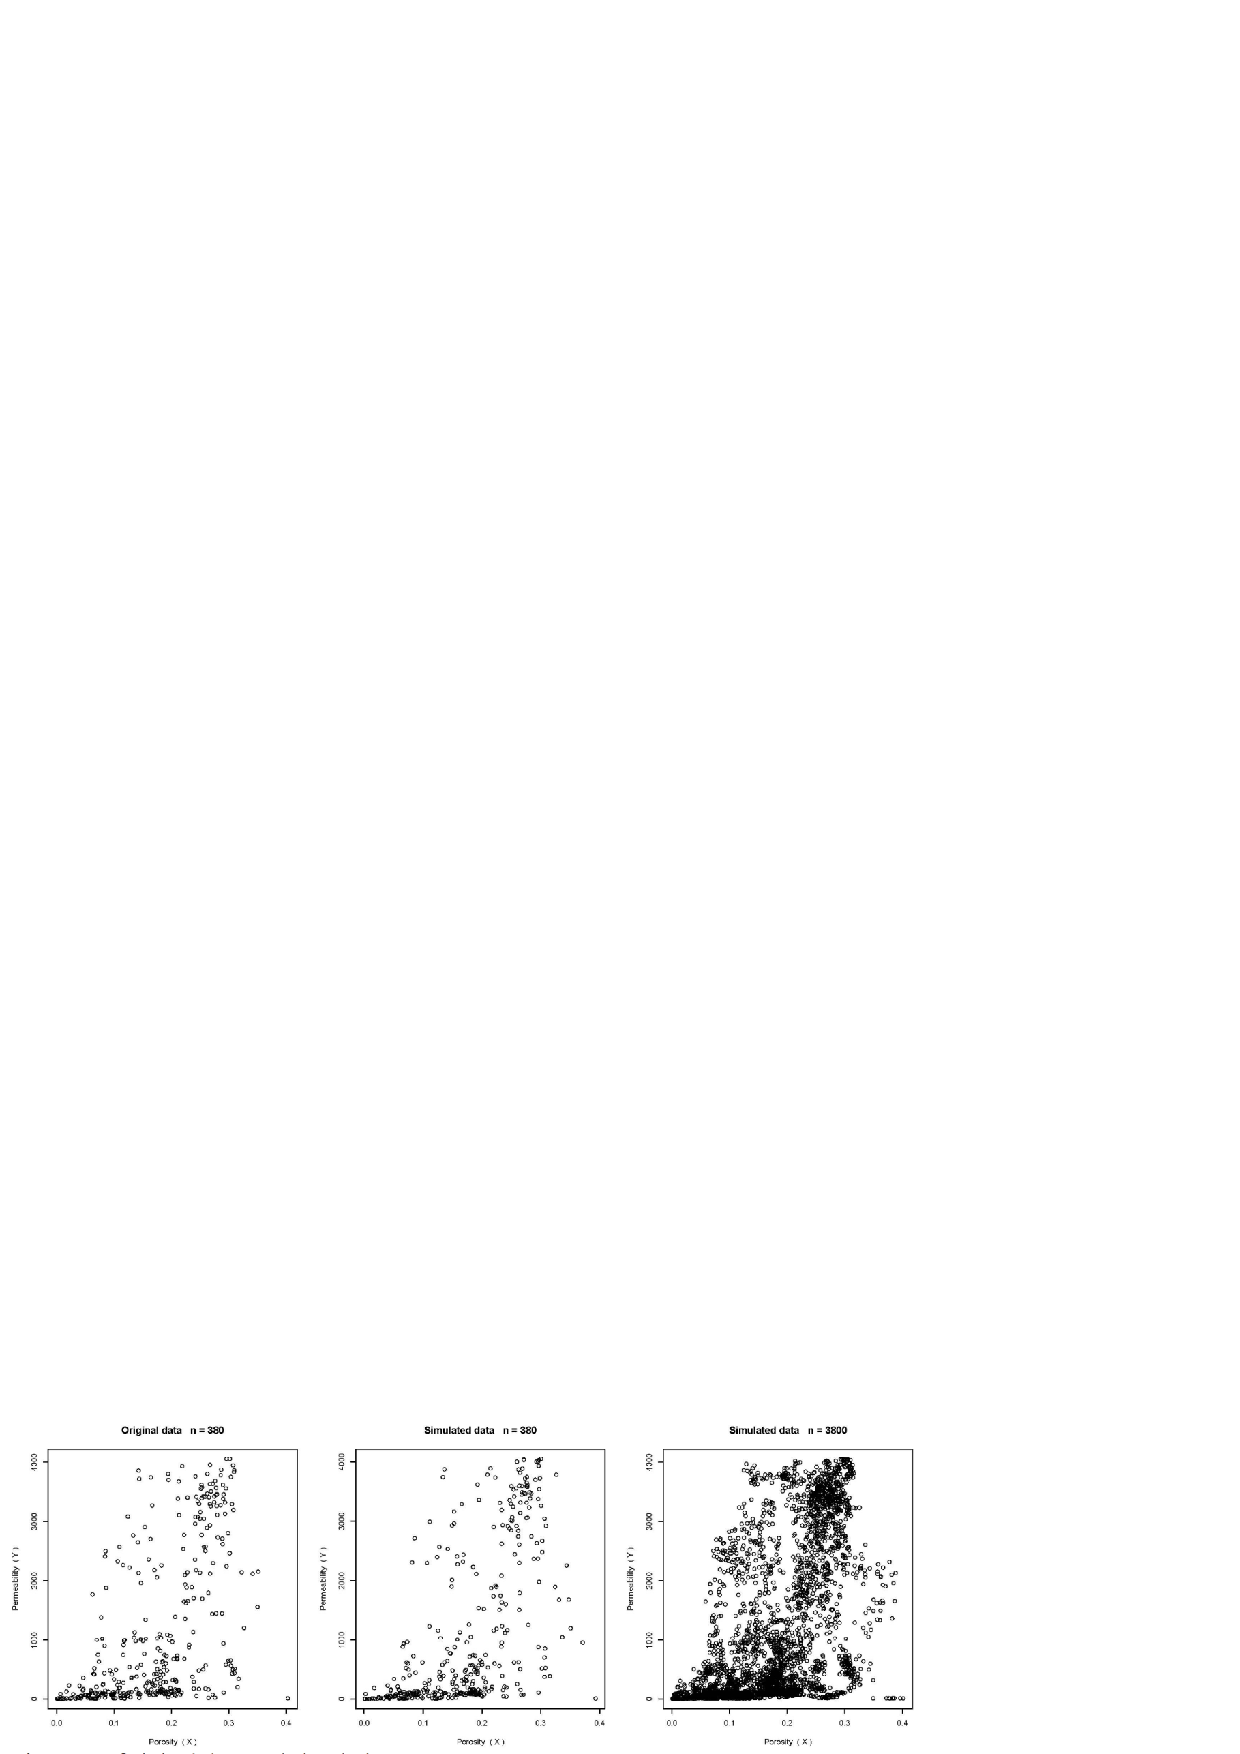
\includegraphics[width=6.14583in,height=2.26042in]{utb5}
	\caption{Ejemplo de la aplicaci\'on de la teor\'ia de c\'opulas de Bernstein \citep{erdely_joint_2012}.}
	\label{f:phiK}
\end{figure}

%donde \({\hat{C}}_{B}\left( \cdot , \cdot \right)\) es la c\'opula emp\'irica definida en la \autoref{e:empCopC}. N\'otese que a diferencia de otros autores \cite{nelsen_introduction_2006} esta definici\'on separa el grado del polinomio de la cantidad de datos, es decir, se puede tener una aproximaci\'on con un polinomio de menor grado, lo que conlleva a simulaciones computacionalmente m\'as r\'apidas.

Para obtener $C_B(u,v)$ se puede utilizar el algoritmo de de'Casteljau o se puede hacer mediante el uso del producto tensorial. Dado que hay suficientes trabajos describiendo el primer enfoque \citep{goldman_pyramid_2002,mann_blossoming_2006}, expliquemos el enfoque mediante tensores \citep{renteln_manifolds_2014} ya que permite una representaci\'on m\'as f\'acil para su implementaci\'on computacional.

\begin{equation}
	C_B(u,v) = \sum \mathbf{A}
\end{equation}	

\noindent
donde hemos definido la notaci\'on $\sum \mathbf{A}$ como la suma de todos los elementos del arreglo $\mathbf{A}$, la cual est\'a definida de la siguiente manera:

\begin{equation}
	\mathbf{A} = 
	\begin{pmatrix}
		\hat{C}(0,0)B(u|0,n)B(v|0,n)  & \hat{C}(0,1)B(u|0,n)B(v|1,n) & \cdots & \hat{C}(0,n)B(u|0,n)B(v|n,n)\\
		\hat{C}(1,0)B(u|1,n)B(v|0,n)  & \hat{C}(1,1)B(u|1,n)B(v|1,n) & \cdots & \hat{C}(1,n)B(u|1,n)B(v|n,n)\\
		\hat{C}(2,0)B(u|2,n)B(v|0,n)  & \hat{C}(2,1)B(u|2,n)B(v|1,n) & \cdots & \hat{C}(2,n)B(u|2,n)B(v|n,n)\\
		\vdots & \vdots & \ddots & \vdots \\
		\hat{C}(n,0)B(u|n,n)B(v|0,n)  & \hat{C}(n,1)B(u|n,n)B(v|1,n) & \cdots & \hat{C}(n,n)B(u|n,n)B(v|n,n)\\
	\end{pmatrix}
\end{equation}

\noindent
tambi\'en definimos $\hat{C}(i,j):= \hat{C}_n (i/n,j/n)$.

Existen varios factores repetidos que se pueden omitir si calculamos los siguientes vectores columna:

\begin{align}
	\mathbf{B}(u|n) &:= (B(u|0,n), B(u|1,n), \ldots, B(u|n,n))^T \\
	\mathbf{B}(v|n) &:= (B(v|0,n), B(v|1,n), \ldots, B(v|n,n))^T
	\label{eq:bernsteinsBasis}
\end{align}

\noindent
y haciendo el producto exterior (o producto tensorial) de dos vectores $\mathbf{a}$ y $\mathbf{b}$, denotado mediante $\mathbf{a} \otimes \mathbf{b}$, el cual produce un matriz $\mathbf{w}$ con coordenadas $w_{ij}= a_i b_j$. Si los vectores son vectores columna, $\mathbf{a} \otimes \mathbf{b}$ es equivalente a la multiplicaci\'on matricial $\mathbf{a}\mathbf{b}^T$. Un ejemplo particular se tiene si $\mathbf{a}=(1,2)^T \in \mathbb{R}^2$ y $\mathbf{b}=(3,4,5)^T \in \mathbb{R}^3$:

\begin{align}
	\mathbf{a} \otimes \mathbf{b}
	=
	\mathbf{a} \mathbf{b}^T
	&=
		\begin{pmatrix}
			a_1 \\ a_2
		\end{pmatrix}
		\begin{pmatrix}
			b_1 & b_2 & b_3
		\end{pmatrix}
	=
		\begin{pmatrix}
			a_1 b_1 & a_1 b_2 & a_1 b_3 \\
			a_2 b_1 & a_2 b_2 & a_2 b_3
		\end{pmatrix} \\
	&=
		\begin{pmatrix}
			1 \\ 2
		\end{pmatrix}
		\begin{pmatrix}
			3 & 4 & 5
		\end{pmatrix}
	=
		\begin{pmatrix}
			1 \cdot 3 & 1 \cdot 4 & 1 \cdot 5 \\
			2 \cdot 3 & 2 \cdot 4 & 2 \cdot 5
		\end{pmatrix}
	=
		\begin{pmatrix}
			3 & 4 & 5 \\
			6 & 8 & 10
		\end{pmatrix}
		\label{e:tensorProd2D}
\end{align}

Por lo tanto, $\mathbf{A}$ se puede reescribir de la siguiente manera:

\begin{equation}
	\mathbf{A}= \hat{\mathbf{C}} \odot [\mathbf{B}(u|n) \otimes \mathbf{B}(v|n)]
\end{equation}

\noindent
donde $\odot$ es el producto elemento-a-elemento de las matrices (tambi\'en conocido como el producto Hadamard o de Schur), y $\hat{\mathbf{C}}$ es la matriz c\'opula emp\'irica (\autoref{e:empCopArray}) cuyos elementos son $\hat{C}_n(u_i,v_j)$. N\'otese que tanto $\mathbf{B}(u|n) \otimes \mathbf{B}(v|n)$ como $\mathbf{\hat{C}}$ pertenecen a $\mathbb{M} ^{(n+1)\times(n+1)}$, las matrices de $(n+1)\times(n+1)$, $n+1$ renglones por $n+1$ columnas.

De esta forma, el c\'odigo computacional se puede hacer eficiente y f\'acil de leer:

\begin{equation}
	C_B(u,v) = \sum \left\{ \mathbf{\hat{C}} \odot [\mathbf{B}(u|n) \otimes \mathbf{B}(v|n)] \right\}
	\label{e:copBernComp}
\end{equation}

M\'as adelante, en la secci\'on de simulaci\'on, se requiere $\partial C_B / \partial u$, la que a su vez requiere las diferencias de primer orden con respecto a $u$ de la c\'opula emp\'irica, $\Delta_u \hat{C}_n$:
	
\begin{equation}
	\Delta_u \hat{C}_n
	\left( \frac{i}{n}, \frac{j}{n} \right)
	= \hat{C}_n
	\left(
		\frac{i+1}{n}, \frac{j}{n}
	\right)
	- \hat{C}_n
	\left(
		\frac{i}{n}, \frac{j}{n}
	\right)
	\label{e:forwardDiff2D}
\end{equation}

Para entender la representaci\'on matricial de la \autoref{e:forwardDiff2D}, a continuaci\'on se muestra un arreglo en el que cada entrada tiene la forma $C_{(i+1)j} - C_{ij}$.

\begin{equation}
\setlength\arraycolsep{8pt}
\Delta_u \mathbf{\hat{C}}=
	\begin{pmatrix}[2]
		C_{10}-C_{00} & C_{11}-C_{01} & C_{12}-C_{02} & \cdots & C_{1n} - C_{0n} \\
		C_{20}-C_{10} & C_{21}-C_{11} & C_{22}-12 & \cdots & C_{2n} - C_{1n} \\ 
		C_{30}-C_{20} & C_{31}-C_{21} & C_{32}-C_{22} & \cdots & C_{3n} - C_{2n} \\ 
		\vdots & \vdots & \vdots & \ddots & \vdots \\
		C_{n0}-C_{(n-1)0} & C_{n1}-C_{(n-1)1} & C_{n2}-C_{(n-1)2} & \cdots & C_{nn} - C_{(n-1)n} \\ 
	\end{pmatrix}
	\label{e:empCopDiffU}
\end{equation}

Este arreglo, se obtiene directamente del arreglo de la c\'opula emp\'irica (\autoref{e:empCopArray}) extendida mediante $C_{0i}=C_{i0}=0$.

\begin{equation}
\setlength\arraycolsep{8pt}
	\mathbf{\hat{C}} =
	\begin{pmatrix}[2]
		C_{00} & C_{01} & C_{02} & C_{03} & \cdots & C_{0(n-1)} & C_{0n}\\
		C_{10} & C_{11} & C_{12} & C_{13} & \cdots & C_{1(n-1)} & C_{1n}\\
		C_{20} & C_{21} & C_{22} & C_{23} & \cdots & C_{2(n-1)} & C_{2n}\\
		C_{30} & C_{31} & C_{32} & C_{33} & \cdots & C_{3(n-1)} & C_{3n}\\
		\vdots  & \vdots  & \vdots  & \vdots  & \ddots & \vdots & \vdots \\
		C_{(n-1)0} & C_{(n-1)1} & C_{(n-1)2} & C_{(n-1)3} & \cdots & C_{(n-1)(n-1)} & C_{(n-1)n}\\
		C_{n0} & C_{n1} & C_{n2} & C_{n3} & \cdots & C_{n(n-1)} & C_{nn}\\
		\end{pmatrix}
	\label{e:empCopArrayExt}
\end{equation}

N\'otese que mientras $\mathbf{\hat{C}} \in \mathbb{M}^{(n+1) \times (n+1)}$, $\Delta_u \mathbf{\hat{C}} \in \mathbb{M}^{n \times (n+1)}$. Al igual que el arreglo de la c\'opula emp\'irica, para ahorrar memoria y evitar errores de redondeo que se puedan propagar a trav\'es de lo c\'alculos, el arreglo $\Delta_u \mathbf{\hat{C}}$ se puede guardar como $\Delta_u n\mathbf{\hat{C}}$ (\autoref{e:empCopArray}).

Por otro lado, tambi\'en es \'util tener a la mano $\Delta_v \mathbf{\hat{C}}$, la diferencia finita de primer orden de la c\'opula emp\'irica con respecto a la segunda variable. En este caso se tiene que $\Delta_u \mathbf{\hat{C}} \in \mathbb{M}^{(n+1) \times n}$ y su arreglo tiene la forma de la \autoref{e:empCopDiffV}. 

\begin{equation}
\setlength\arraycolsep{8pt}
\Delta_v \mathbf{\hat{C}}=
	\begin{pmatrix}[2]
		C_{01}-C_{00} & C_{02}-C_{01} & C_{03}-C_{02} & \cdots & C_{0n} - C_{0(n-1)} \\
		C_{11}-C_{10} & C_{12}-C_{11} & C_{13}-C_{12} & \cdots & C_{1n} - C_{1(n-1)} \\ 
		C_{21}-C_{20} & C_{22}-C_{21} & C_{23}-C_{22} & \cdots & C_{2n} - C_{2(n-1)} \\ 
		C_{31}-C_{30} & C_{32}-C_{31} & C_{33}-C_{32} & \cdots & C_{3n} - C_{3(n-1)} \\ 
		\vdots & \vdots & \vdots & \ddots & \vdots \\
		C_{n1}-C_{n0} & C_{n2}-C_{n1} & C_{n3}-C_{n2} & \cdots & C_{nn} - C_{n(n-1)} \\ 
	\end{pmatrix}
	\label{e:empCopDiffV}
\end{equation}

Ahora, estamos preparados para definir las derivadas de la c\'opula de Bernstein \citep{phillips_interpolation_2003,sancetta_bernstein_2004}:

\begin{align}
	\partial C_B / \partial u
	&= \sum_{j=0}^n
	\left\{
		B(v|j,n) n 
		\left[
			\sum_{i=0}^{n-1} \Delta_u \hat{C}_n 
			\left(
				\frac{i}{n} , \frac{j}{n}
			\right)
			B(u|i,n-1)
		\right]
	\right\} \\
	&= n \sum_{i=0}^{n-1} \sum_{j=0}^n B(u|i,n-1) \Delta_u \hat{C}_n 
	\left(
		\frac{i}{n} , \frac{j}{n}
	\right)
	B(v|j,n) 
	\label{eq:bernsCopDerU}
\end{align}

Los sumandos de esta ecuaci\'on, al igual que para la c\'opula de Bernstein (\autoref{e:empCopArray}), se pueden escribir como elementos de la matriz de la \autoref{eq:empCopDiffUarray}:

\begin{equation}
	\begin{pmatrix}
		B(u|0,n-1)\Delta_u \hat{C}_n(0,0)B(v|0,n) & \cdots & B(u|0,n-1)\Delta_u \hat{C}_n(0,1)B(v|n,n) \\
		B(u|1,n-1)\Delta_u \hat{C}_n(\frac{1}{n},0)B(v|0,n) & \cdots & B(u|1,n-1)\Delta_u \hat{C}_n(\frac{1}{n},1)B(v|n,n) \\
		B(u|2,n-1)\Delta_u \hat{C}_n(\frac{2}{n},0)B(v|0,n) & \cdots & B(u|2,n-1)\Delta_u \hat{C}_n(\frac{2}{n},1)B(v|n,n) \\
		\vdots & \ddots & \vdots \\
		B(u|n-1,n-1)\Delta_u \hat{C}_n(\frac{n-1}{n},0)B(v|0,n) & \cdots & B(u|n-1,n-1)\Delta_u \hat{C}_n(\frac{1}{n},1)B(v|n,n) \\
	\end{pmatrix}
	\label{eq:empCopDiffUarray}
\end{equation}

Reutilizando la \autoref{eq:bernsteinsBasis} y la \autoref{e:empCopDiffU}, tenemos que

\begin{equation}
	\frac{\partial C_B}{\partial u}(u,v)
	= n \sum \left\{\Delta_u \mathbf{\hat{C}} \odot [\mathbf{B}(u|n-1) \otimes \mathbf{B}(v|n)] \right\}
	\label{e:copBernDiffComp}
\end{equation}

De manera similar tenemos:

\begin{equation}
	\frac{\partial C_B}{\partial v}(u,v)
	= n \sum \left\{\Delta_v \mathbf{\hat{C}} \odot [\mathbf{B}(u|n) \otimes \mathbf{B}(v|n-1)] \right\}
	\label{e:copBernDiffVComp}
\end{equation}

La funci\'on de densidad de c\'opula $c$ ($c$ min\'uscula) es la segunda derivada parcial con respecto a cada una de las variables. En el caso de la c\'opula de Bernstein, \'esta se puede escribir como \citep{carnicero_non-parametric_2013}:

\begin{equation}
	\hat{c}_{B} (u,v)
	= \sum_{i = 0}^{n} {\sum_{j = 0}^{n} p_{i j}}
	\beta \left( u|i,n-i+1 \right)
	\beta \left( v|j,n-j+1 \right)
	\label{eq:bernsCopDens2D}
\end{equation}

Donde

\begin{equation*}
	\beta (x|a,b) = \frac{1}{B(a,b)} x^{a-1} (1-x)^{b-1}
\end{equation*}

\noindent
Y donde los pesos son

\begin{equation}
	p_{ij} = \frac{1}{n}\sum_{k=1}^{n}
	\mathbbm{1}
	\left(
	\frac{i-1}{n} < u_k \le \frac{i}{n},
	\frac{j-1}{n} < v_k \le \frac{j}{n}
	\right)
	\label{eq:copWeights}
\end{equation}

\noindent
Para $i,j = 1,\ldots,n$.

Estos pesos son equivalentes al estimador del histograma en $[0,1]^2$ de la c\'opula (para m\'as detalle de dichos estimadores v\'ease \cite{scott_multivariate_1992}); es decir, $p_{ij}$  es $1/n$ veces el n\'umero de puntos $(u_i, v_i)$ dentro del rect\'angulo delimitado por el rect\'angulo $(i-1,i]/k \times (j-1,j]/k$ (v\'ease \autoref{fig:periodicCondition}).

\begin{figure}[H]
	\centering
	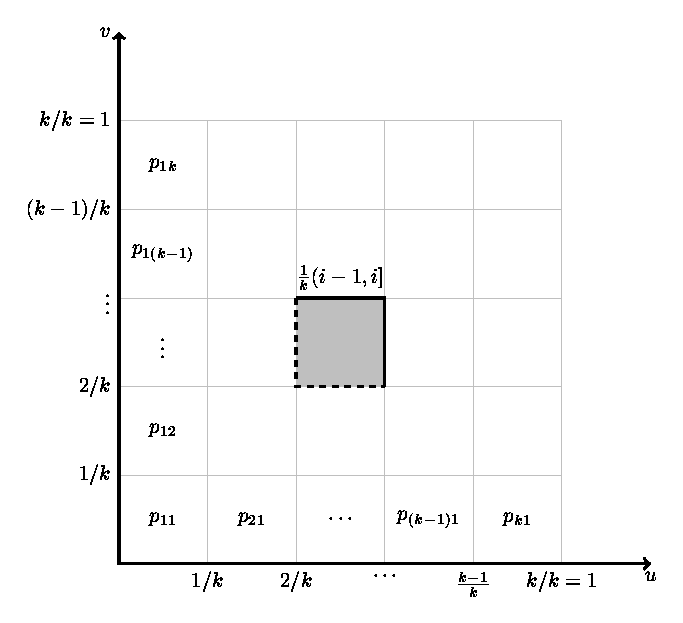
\includegraphics{periodicCondition}
	\caption{Representaci\'on esquem\'atica de los pesos $p_{ij}$ de la densidad de c\'opula.}
	\label{fig:periodicCondition}
\end{figure}

\cite{sancetta_bernstein_2004} y \cite{phillips_interpolation_2003} demuestran que el sesgo de los polinomios Bernstein de orden \(k\) es del orden de\(\ d \slash k + \mathcal{O}(1 \slash k)\) para alguna constante finita \(d\). Ellos tambi\'en proporcionan valores \'optimos para \(k\).

Recientemente el uso de splines penalizados se ha incorporado a la teor\'ia de c\'opulas no param\'etricas \cite{kauermann_flexible_2013}. En dicho trabajo se muestra las ventajas que tienen los splines penalizados sobre otros enfoques no param\'etricos como el de Bernstein, wavelets y kernel. \cite{kauermann_flexible_2013} aproximan la copula densidad, \(c\),

\[c\left( u_{1},\ldots,u_{p} \right) \approx \sum_{\mathbf{k}\mathcal{\in K}}^{}{b_{\mathbf{k}}\phi_{\mathbf{k}}\left( u_{1},\ldots,u_{p} \right)}\]

\noindent
Donde \(b_{\mathbf{k}}\) son los coeficientes y \(\phi_{\mathbf{k}}\)
son splines penalizados.

\section{C\'opulas bivariadas para vectores aleatorios con componentes orientadas}\label{s:copCirLin}

\cite{johnson_angular-linear_1978,wehrly_bivariate_1980} mostraron que la
funci\'on de distribuci\'on conjunta de una variable \(X\), y una
circular \(\Theta\), se puede expresar como

$$f_{\Theta,X}\left( \theta,x \right) = 2\pi g \{ 2\pi\left\lbrack F_{\Theta}\left( \theta \right) + F_{X}\left( x \right) \right\rbrack \} f_{\Theta}\left( \theta \right)f_{X}\left( x \right)$$

Donde \(g\left( \cdot \right)\) es una funci\'on de densidad de una
variable aleatoria circular. Por lo tanto, la copula para \(\Theta\) y
\(X\) debe satisfacer:

$$c\left( F_{\Theta}\left( \theta \right),F_{X}\left( x \right) \right) = 2\pi g\left( 2\pi\left\lbrack F_{\Theta}\left( \theta \right) + F_{X}\left( x \right) \right\rbrack \right)$$

Una de las aplicaciones de esta teor\'ia se ha hecho en la estimaci\'on de ozono en la ciudad de M\'exico \cite{fernandezduran_modelling_2004} usando sumas trigonom\'etricas no negativas para modelar la funci\'on de densidad de variables aleatorias circulares y c\'opulas circulares-lineales para modelar la dependencia conjunta. N\'otese que el enfoque de Fern\'andez-Dur\'an es un enfoque param\'etrico.

Otro caso de c\'opulas no param\'etricas de datos que incluyen datos circulares es la adaptaci\'on de \cite{carnicero_non-parametric_2013} a las c\'opulas de Bernstein de \cite{sancetta_bernstein_2004}. Dicha adaptaci\'on consiste en modelos propuestos para tomar en cuenta la periodicidad de los datos circulares.

La funci\'on de densidad de probabilidad \(f_{\Theta,X}\left( \cdot , \cdot \right)\) de un vector aleatorio \(\left( \Theta,X \right)\) es una funci\'on no negativa definida en la superficie de un cilindro \(\mathbb{S}^{1}\mathbb{\times R}\). Esta densidad tiene periodo \(2\pi\) en la componente circular:

\begin{equation}
	f_{\Theta,X}\left( \theta,x \right) = f_{\Theta,X}\left( \theta + 2k,x \right)
	\label{eq:periodiccondition}
\end{equation}

\noindent
para \(k \in \mathbb{Z}, -\infty < \theta < \infty\),

Y su integral es uno sobre un intervalo de longitud \(2\pi\) por los reales. Es decir, se integra a uno en todo su dominio.

Como consecuencia del teorema de \cite{sklar_fonctions_1959},

$$f_{\Theta,X}\left( \theta,x \right) = c\left( F_{\Theta}\left( \theta \right),F_{X}\left( x \right) \right)f_{\Theta}\left( \theta \right)f_{X}\left( x \right)$$

\noindent
donde \(c\left( \cdot , \cdot \right)\) es la densidad c\'opula.

Debido a la condici\'on de periodicidad para la funci\'on de distribuci\'on conjunta (\autoref{eq:periodiccondition}, es necesario que la c\'opula satisfaga:

\begin{equation}
	c\left( 0,v \right) = c\left( 1,v \right) \qquad \forall v \in [0,1]
	\label{eq:periodCop}
\end{equation}

Las c\'opulas de Bernstein no cumplen esta condici\'on, para la cual es necesario que los pesos de la \autoref{eq:copWeights}  satisfagan \(p_{1j_{2}} = p_{kj_{2}}\) para\(j_{2} = 1,\ldots,k\). Para remediarlo, \citet{carnicero_non-parametric_2013} proponen,

\begin{align}
	\tilde{p}_{1j_{2}} = {\tilde{p}}_{kj_{2}} = \frac{p_{1j_{2}} + p_{kj_{2}}}{2}  \qquad j_{2} &= 1,\ldots,k \label{eq:bernsWper}\\
	{\tilde{p}}_{j_{1}j_{2}} = p_{j_{1}j_{2}} \qquad j_{1} &\neq 1,k
\end{align}

Partiendo de la \autoref{fig:periodicCondition}, la correcci\'on de la \autoref{eq:bernsWper} equivale a promediar los vectores de pesos \verb|p[1,:]| y \verb|p[k,:]|. De manera visual, dicha correcci\'on se obtiene al promediar las dos celdas del mismo tono de gris en la \autoref{fig:periodicConditionCorrection}.

\begin{figure}
	\centering
	\includegraphics{periodicConditionCorrection}
	\caption{Correcci\'on para que la c\'opula de Bernstein cumpla con la condici\'on de periodicidad en la primera variable (\autoref{eq:periodCop}).}
	\label{fig:periodicConditionCorrection}
\end{figure}

Para validar el software desarrollado en \verb|R| se reprodujeron los resultados del art\'iculo de \citet{carnicero_non-parametric_2013} en el que se muestra la aplicaci\'on de esta metodolog\'ia a datos de direcci\'on del viento y precipitaci\'on pluvial. Para tal objetivo, se estimaron las funciones de densidad de probabilidad univariada para ambos datos. Para la direcci\'on del viento la funci\'on de densidad univariada fue una combinaci\'on de tres distribuciones de von Mises y para los datos de precipitaci\'on la funci\'on de densidad se compone de una combinaci\'on de tres exponenciales (\autoref{f:gijonDenCT}).

\begin{figure}
	\centering
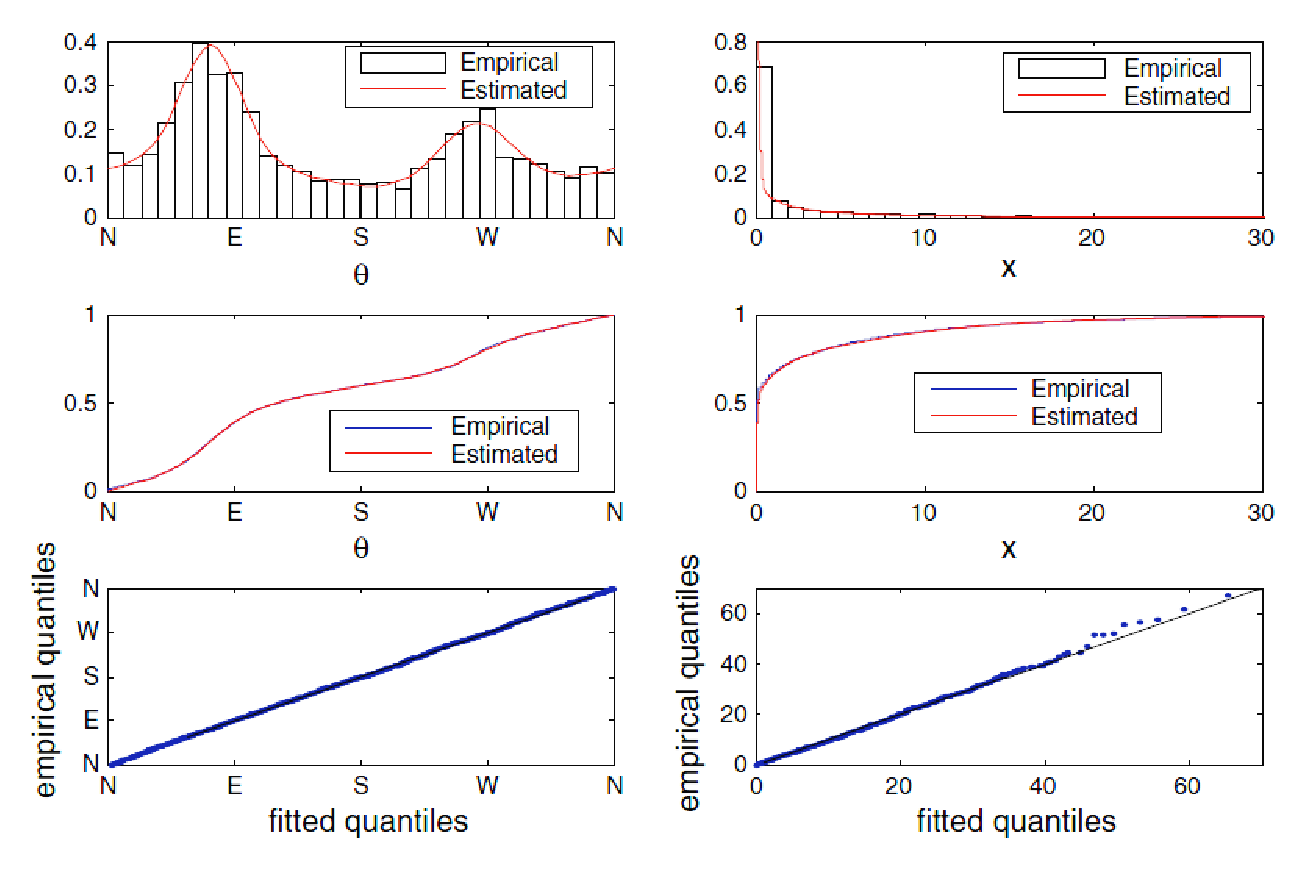
\includegraphics[width=5.01249in,height=3.32350in]{utb7}
	\caption{Densidad marginal estimada (top), funci\'on de distribuci\'on (medio) y gr\'aficos de cuantiles (abajo) para direcci\'on del viento (izquierda) y para la precipitaci\'on pluvial (derecha). Tomada de \cite{carnicero_non-parametric_2013}.}
	\label{f:gijonDenCT}
\end{figure}

Para estimar la funci\'on de densidad conjunta se utiliza la metodolog\'ia mostrada en esta secci\'on en lo que respecta a la parte bivariada. En la parte univariada aqu\'i proponemos que sea mediante los polonimos de Bernstein-Kantorovich, pero para reproducir los resultados de \citet{carnicero_non-parametric_2013} se utilizaron los modelos que ellos ajustaron. El resultado se muestra en la \autoref{f:gijonJointDens} y en la \autoref{f:gijonDenCT}. N\'otese que las marginales son claramente respetadas y la funci\'on de densidad es peri\'odica con respecto a la variable aleatoria orientada.

\begin{figure}[H]
	\centering
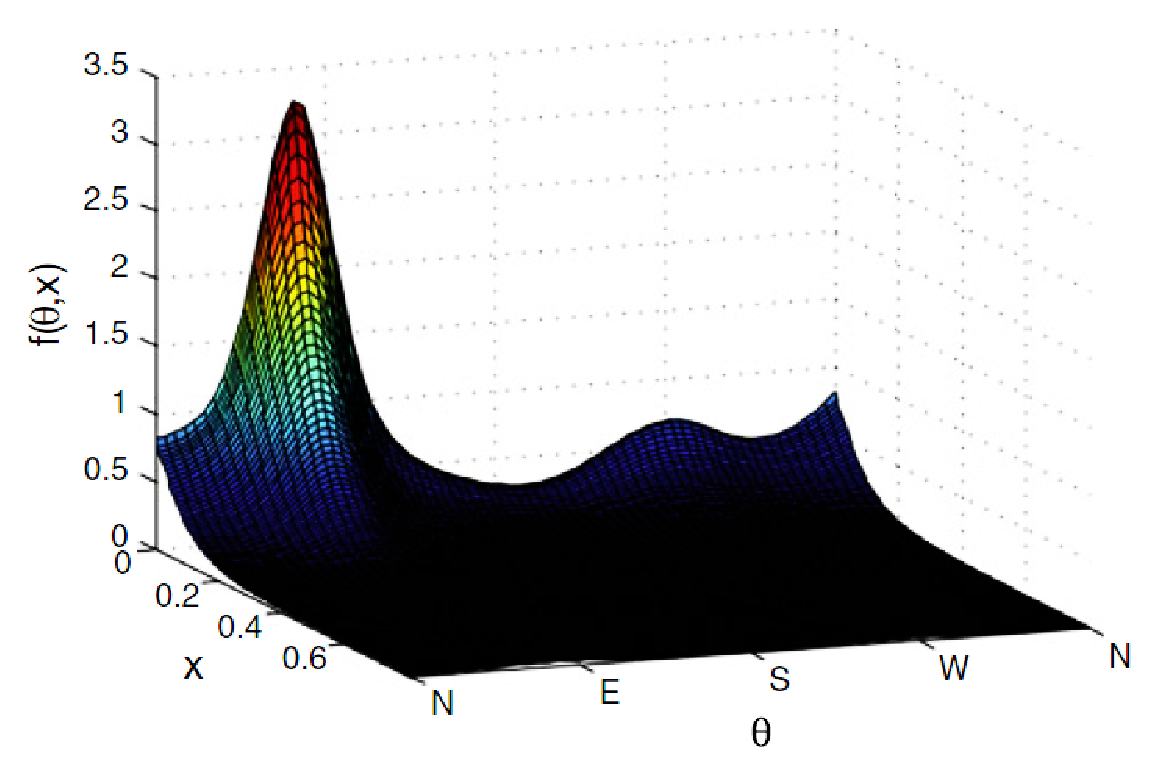
\includegraphics[width=3.75000in,height=2.47917in]{utb8}
	\caption{Funci\'on de densidad conjunta estimada (utilizando c\'opulas de Bernstein) de la variable circular-lineal \(\left( \Theta,X \right)\) . La cual describe la direcci\'on del viento y la precipitaci\'on pluvial.}
	\label{f:gijonJointDens}
\end{figure}

N\'otese que, aunque la correcci\'on propuesta por \citet{carnicero_non-parametric_2013} permite una c\'opula continua, no asegura diferenciabilidad, es decir, no asegura que la c\'opula sea suave en las fronteras. Una opci\'on m\'as vers\'atil que los polinomios de Bernstein que permite modelar curvas y sus derivadas al mismo tiempo son los splines. Dado que la suavidad se pide en la densidad, el enfoque de c\'opulas con splines propuesto por \citet{schellhase_density_2012} o el de Ferreira (2008 directional logspline) puede ser \'util para una aproximaci\'on m\'as natural en el caso de vectores aleatorios con componentes circulares.

%\section{C\'opulas no param\'etricas para datos circulares-circulares}\label{s:copParDir}

Hasta este momento solamente se ha estudiado el caso con una sola componente circular, pero m\'as es posible. En el caso bivariado, se puede hacer que ambas componentes sean circulares.

La funci\'on de densidad de probabilidad \(f_{\Theta_{1},\Theta_{2}}\left( \cdot , \cdot \right)\) de un vector aleatorio circular-circular \(\left( \Theta_{1},\Theta_{2} \right)\) es una funci\'on no negativa definida en la superficie de un toro, \(\mathbb{S}^{1} \times \mathbb{S}^{1}\). Esta densidad tiene periodo \(2\pi\) en ambas componentes:

\begin{equation}
f_{\Theta_{1},\Theta_{2}}\left( \theta_{1},\theta_{2} \right) = f_{\Theta_{1},\Theta_{2}}(\theta_{1} + 2j\pi,\theta_{2} + 2k\pi), \qquad j,k\mathbb{\in Z}, - \infty < \theta_{1},\theta_{2} < \infty 
\label{eq:den2Dcir}
\end{equation}
Y su integral es uno sobre el producto de dos intervalos de longitud \(2\pi\). Es decir, es uno al integrar sobre todo su dominio.

Debido a la condici\'on (\autoref{eq:den2Dcir}) para la funci\'on de distribuci\'on conjunta, es necesario que la c\'opula para datos circulares-circulares, adem\'as de la \autoref{eq:periodCop}, satisfaga:

\begin{equation}
	c(u,0) = c(u,1) \qquad \forall u \in [0,1]
	\label{eq:periodCondition2D}
\end{equation}

En el caso de las c\'opulas de Bernstein, los pesos son similares a la \autoref{eq:copWeights} salvo que las dos variables aleatorias correspondientes son circulares.
Por lo tanto los pesos tienen que satisfacer $p_{1j_{2}} = p_{kj_{2}}\) y \(p_{j_{1}1} = p_{j_{1}k}$ para $j_{1},j_{2} = 1,..,k$.
Y la correcci\'on de periodicidad, adem\'as de aplicarse a la primera variable $u$, posteriormente tiene que aplicarse a la segunda variable $v$. Lo que produce los siguientes pesos:

\({\tilde{p}}_{1j_{2}} = {\tilde{p}}_{kj_{2}} = \frac{p_{1j_{2}} + p_{kj_{2}}}{2}\)

\({\tilde{p}}_{j_{1}1} = {\tilde{p}}_{j_{1}k} = \frac{p_{j_{1}1} + p_{j_{1}k}}{2}\)

\({\tilde{p}}_{11} = {\tilde{p}}_{1k} = {\tilde{p}}_{k1} = {\tilde{p}}_{\text{kk}} = \frac{p_{11} + p_{1k} + p_{k1} + p_{\text{kk}}}{4}\)

Y \({\tilde{p}}_{j_{1}j_{2}} = p_{j_{1}j_{2}}\) para \(j_{1} \neq 1,k\)
y \(j_{2} \neq 1,k\) 

Lo que garantiza que la c\'opula se continua y peri\'odica en ambas variables.

Para ilustrar la metodolog\'ia, \cite{carnicero_non-parametric_2013} muestra la aplicaci\'on de esta metodolog\'ia a datos de direcci\'on dos boyas en el mar. Para tal objetivo, se estimaron las funciones de densidad de probabilidad univariada para ambos datos. En ambas variables, la funci\'on de densidad univariada fue una combinaci\'on de tres distribuciones de von Mises (\autoref{f:marginalDir}).

\begin{figure}[H]
	\centering
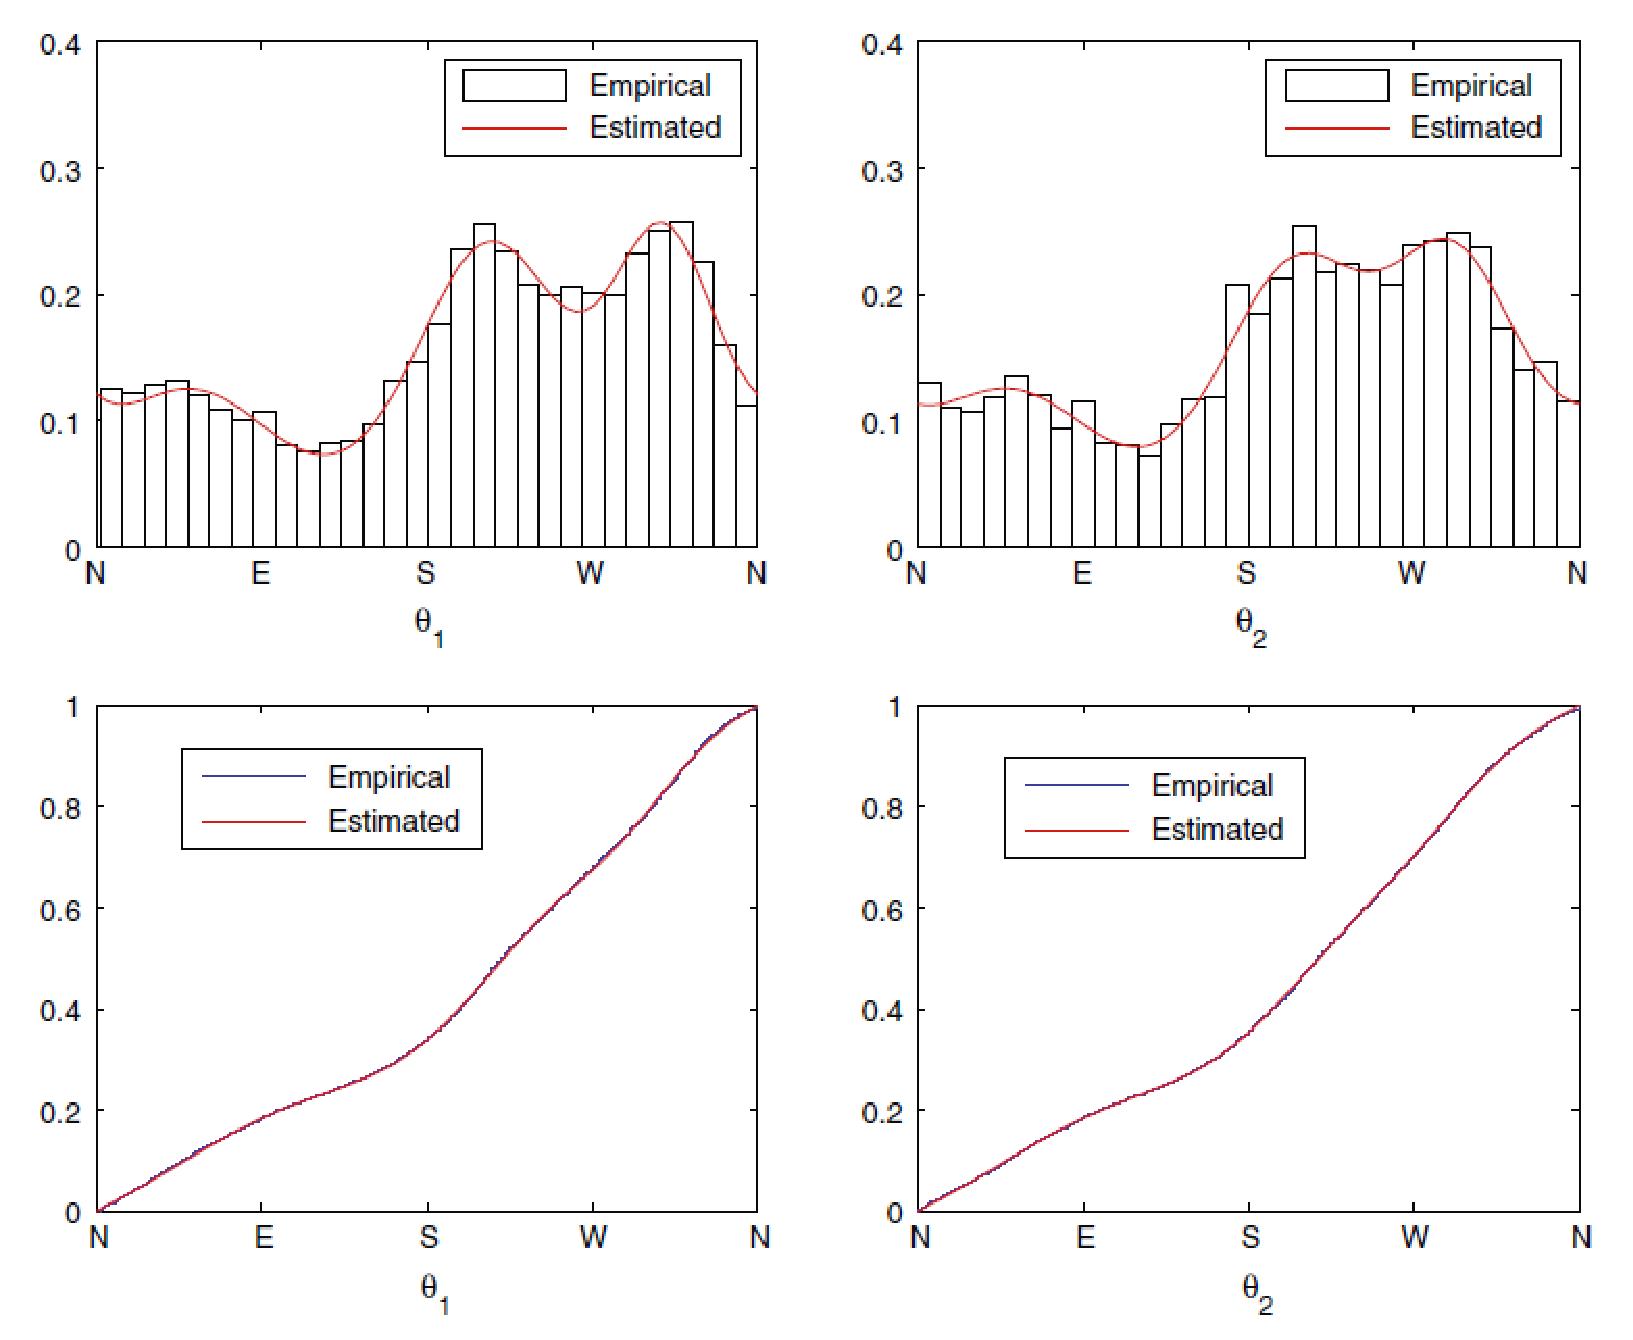
\includegraphics[width=4.82292in,height=3.93750in]{utb9}
	\caption{Densidad marginal estimada (top) y funci\'on de distribuci\'on (abajo) para la direcci\'on de dos boyas.}
	\label{f:marginalDir}
\end{figure}

\section{Simulaci\'on conjunta de variables aleatorias: caso bivariado}\label{s:simAlg2D}

Dado un modelo de dependencia (c\'opula), uno de los objetivos perseguidos al modelar la funci\'on de densidad de probabilidad conjunta es simular valores de las variables aleatorias.
Para simular datos a partir de la c\'opula se utiliza una variante del m\'etodo de distribuci\'on condicional \citep{nelsen_introduction_2006} en el cual se utiliza un enfoque no param\'etrico \citep{erdely_nonparametric_2009,erdely_joint_2012}:

\begin{enumerate}
\item
  Genere dos variables aleatorias \(u\) y \(t\) que sean independientes   y continuas en \(\left( 0,1 \right)\).
\item
  Obtenga \(v = c_{u}^{\left( - 1 \right)}\left( t \right)\). Donde
  \(t = c_{u}\left( v \right) = \frac{\partial\tilde{C}\left( u,v \right)\ }{\partial u}\)
  y \(c_{u}^{\left( - 1 \right)}\) es la inversa generalizada (\autoref{e:generalizedInv}) de \(c_{u}\).
\item
	Los datos simulados, \(\left( x,y \right)\), se obtienen utilizando   funciones cuantiles no param\'etricas de \(X\) y \(Y\) respectivamente.   Estas funciones \(\tilde{Q}\) y \(\tilde{R}\) son estimadas mediante   polinomios de Bernstein-Kantorovich \citep{munoz-perez_estimating_1987}. Por lo tanto   \(\left( x,y \right) = \left( \tilde{Q}\left( u \right),\tilde{R}\left( v \right) \right)\).
\end{enumerate}

Atendiendo al punto 1 de esta metodolog\'ia es necesario simular valores con una distribuci\'on uniforme en el intervalo \(\left\lbrack 0,1 \right\rbrack\), ya que estos son requeridos por la c\'opula. Esto se puede conseguir con la funci\'on \verb|stats::runif|. Recu\'erdese que la c\'opula bivariada tiene dominio \(\left\lbrack 0,1 \right\rbrack^{2}\).
Para el segundo paso se requieren a) la  derivada parcial de la c\'opula; b) obtener una funci\'on inversa.
En el caso de la c\'opula de Bernstein la derivada est\'a dada por la \autoref{eq:bernsCopDerU}.
Al terminar este segundo paso se cuenta con dos valores $u_i$ y $v_i$ que est\'an distribuidos uniformemente pero que conservan la misma dependencia que los datos originales.
Por \'ultimo, estos valores son los argumentos de las funciones cuantiles para obtener $x_i$ y $y_i$. 
La implementaci\'on computacional de estas funciones cuantiles se encuentra en el paquete \verb|lmomco| bajo el nombre de \verb|dat2bernqua|.
La \autoref{f:phiKhist} muestra un ejemplo de un conjunto de datos a los cuales se les model\'o su funci\'on de distribuci\'on con los polinomios de Bernstein-Kantorovich. Por lo tanto
$(x_{i},y_{i}) = (\tilde{Q}(u_{i}), \tilde{R}(v_{i}))$.

\begin{figure}[H]
	\centering
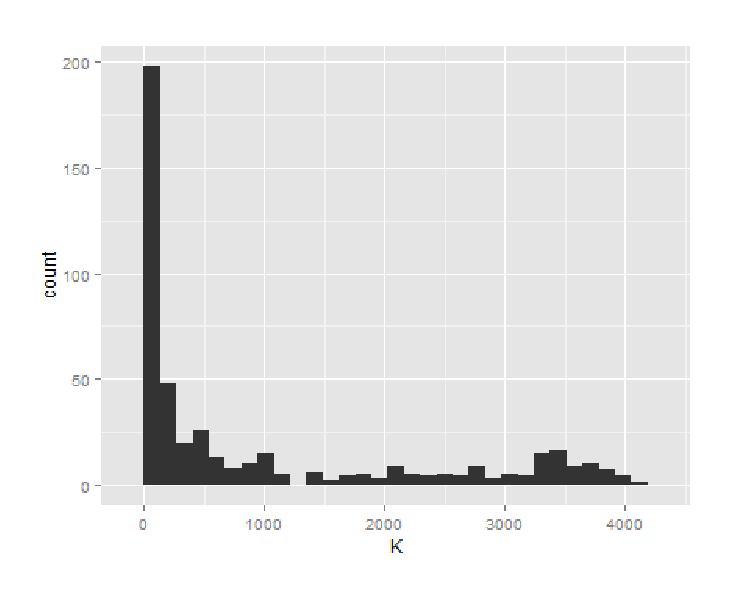
\includegraphics[width=2.82000in,height=2.24000in]{utb13}
\includegraphics[width=2.82000in,height=2.24000in]{utb14}
\caption{Histogramas de un ejemplo de simulaci\'on no param\'etrica. 473 datos (izquierda) y 100 datos simulados (derecha).}
\label{f:phiKhist}
\end{figure}

\section{Simulaci\'on conjunta de variables aleatorias: caso multivariado}

Uno de los objetivos al modelar vectores aleatorios es generar muestras estad\'{i}sticamente equivalentes a los datos observados para as\'{i} poder cuantificar incertidumbre. Para lograr este cometido, se ilustra el algoritmo de simulaci\'{o}n.

El algoritmo de simulaci\'{o}n se simplifica si todas las $d$ marginales unidimensionales se distribuyen uniformemente lo cual se logra obteniendo la funci\'{o}n de distribuci\'{o}n acumulada de los datos ya que $F_i(x_i) \sim Uniforme(0,1)$. La generalidad del algoritmo se recupera al mapear cada marginal $u_{i} := F(x_i)$ en su variable correspondiente $x_{i}$ mediante el m\'etodo de la transformada inversa \citep[sec. 2.1.2, pp. 44]{robert_introducing_2009} utilizando la inversa generalizada (\autoref{e:generalizedInv}.

Para obtener una muestra simulada se procede con el siguiente algoritmo recursivo (\citeauthor{mai_simulating_2012}, \citeyear{mai_simulating_2012}, sec. 5.3.2, pp. 208;\citeauthor{dismann_statistical_2010}, \citeyear{dismann_statistical_2010}):

\begin{align}
	\text{inicio:} \qquad  W_{i} & \overset{i.i.d.}{\sim} Uniforme(0,1), \qquad \forall i \in \{1, \ldots, d\} \\
	\text{posteriormente:} \qquad U_{1} &:= W_{1} \\
U_{2} &:= F_{2|1}^{-}(W_{2}|U_{1}) \\
U_{3} &:= F_{3|2,1}^{-}(W_{3}|U_{2}, U_{1}) \\
% todo: insert vertical dots (ellipsis) here
U_{d} &:= F_{d|d - 1, \ldots, 1}^{-}(W_{d}|U_{d-1}, \ldots, U_{1})
\label{e:CopSimAlg_multi}
\end{align}

En el caso de teor\'ia de c\'opulas cada $F^{-}_{i|i-1,\ldots,1}$ es la inversa generalizada de la \autoref{e:CondDistVine}.

\section{Vine c\'{o}pulas: Caso trivariado}

Es bien sabido que el an\'{a}lisis y visualizaci\'{o}n bivariado de datos es m\'{a}s f\'{a}cil que el caso multivariado. Esto tambi\'en se cumple en el caso de la modelaci\'{o}n de dependencias mediante c\'{o}pulas. Un enfoque que permite estudiar dependencias con $d \ge 3$ mediante descomposiciones bivariadas es el conocido como Vine copulas (tambi\'en conocido como construcciones de c\'{o}pulas mediante pares).

El siguiente caso trivariado ilustra c\'{o}mo se efect\'{u}a la descomposici\'{o}n en pares a partir de la funci\'{o}n de densidad conjunta $f_{123}$ \citep{diaz2015vine}:

\begin{align}
f_{123} &= f_{23|1} \cdot f_1 \\
 &=c_{23|1} (F_{2|1}, F_{3|1}) \cdot f_{2|1} \cdot f_{3|1} \cdot f_1 \\
 &=c_{23|1} (F_{2|1}, F_{3|1}) \cdot \frac{f_{12}}{f_1} \cdot \frac{f_{13}}{f_1} \cdot f_1 \\
 &=c_{23|1} (F_{2|1}, F_{3|1}) \cdot c_{12}(F_1, F_2) \cdot c_{13}(F_1, F_3) \cdot f_1 \cdot f_2 \cdot f_3
\label{e:vine3}
\end{align}

N\'{o}tese que para la misma densidad $f_{123}$ existen otras dos posibles descomposiciones dependiendo de la variable condicionante.

Cada uno de los argumentos de las c\'opulas bivariadas de la descomposici\'on Vine (ecuaci\'on \ref{e:vine3}) est\'a dado como \citep{mai_simulating_2012,aas_pair-copula_2009,dismann_statistical_2010}:
%(\citeauthor{mai_simulating_2012}, \citeyear{mai_simulating_2012}, pp. 189, eq. 5.7). 
%; \citeauthor{gijbels_conditional_2011}, \citeyear{gijbels_conditional_2011}

\begin{equation}
F(x| \mathbf{x}) = \frac{\partial C_{X,X_j|\mathbf{X}_{-j}}
(F(x|\mathbf{x}_j), F(x_j|\mathbf{x}_{-j})}
{F(x_j|\mathbf{x}_{-j})}
\label{e:CondDistVine}
\end{equation}

\noindent
donde $\mathbf{x} \subset \{x_1, \ldots, x_d \}$, $\mathbf{x}^c:= \{x_1,\ldots, x_d\} - \mathbf{x}$, $x \notin \mathbf{x}$  y $x_j \notin \mathbf{x}_j \subset \mathbf{x}$.

N\'{o}tese que en la ecuaci\'{o}n (\ref{e:CondDistVine}) se utilizan may\'{u}sculas para denotar variables aleatorias mientras que las min\'{u}sculas denotan observaciones (realizaciones). La notaci\'{o}n tambi\'en distingue entre escalares ($x$ \'{o} $X$) y vectores ($\mathbf{x}$).

Para el caso trivariado se tiene \citep[pp. 209, example 5.7]{mai_simulating_2012} 

\begin{equation}
F(u_3| u_1,u_2) = \frac{\partial C_{3,1|2}
(F(u_3|u_2), F(u_1|u_2)}
{\partial F(u_1|u_2)}
\label{e:CondDistVine3}
\end{equation}

Un caso particular de las c\'opulas de Vine se tiene haciendo el \textit{supuesto de simplificaci\'on} \citep{joe_dependence_2014,gijbels_conditional_2011}

\begin{equation}
C_{3,1|2} = C_{3,1}
\label{e:simpAssum} % simplifying assumption
\end{equation}

Un caso m\'as particular pero frecuente se tiene si $U_3 \perp U_1 | U_2$ (ver \ref{e:IndCop}):

\begin{equation}
C_{3,1|2} (u,w) = uw
\label{e:CondInd} % conditionally independent copula
\end{equation}

Utilizando \ref{e:CondInd} en \ref{e:CondDistVine3} se tiene:

\begin{equation}
\frac{\partial C_{3,1|2}}{\partial F(u_1|u_2)} = F(u_3|u_2)
\label{e:marginalInd} % Marginally independent
\end{equation}

Lo que reduce el tiempo de c\'omputo para la simulaci\'on.

%N\'{o}tese que a cada par $F_{x|x} -- C_{x}$ correspondiente a la ecuaci\'{o}n MISSING, en el \'{a}rbol, se cuenta con dos argumentos de entrada (n\'{o}dos-hijos) y un argumento de salida $u_{i}$.
%
%En el \'{a}rbol se distingue entre nodo-hijo izquierdo y derecho. N\'{o}tese que en este caso particular, los nodos-hijos izquierdos corresponden con valores $w_{i}$.
%
%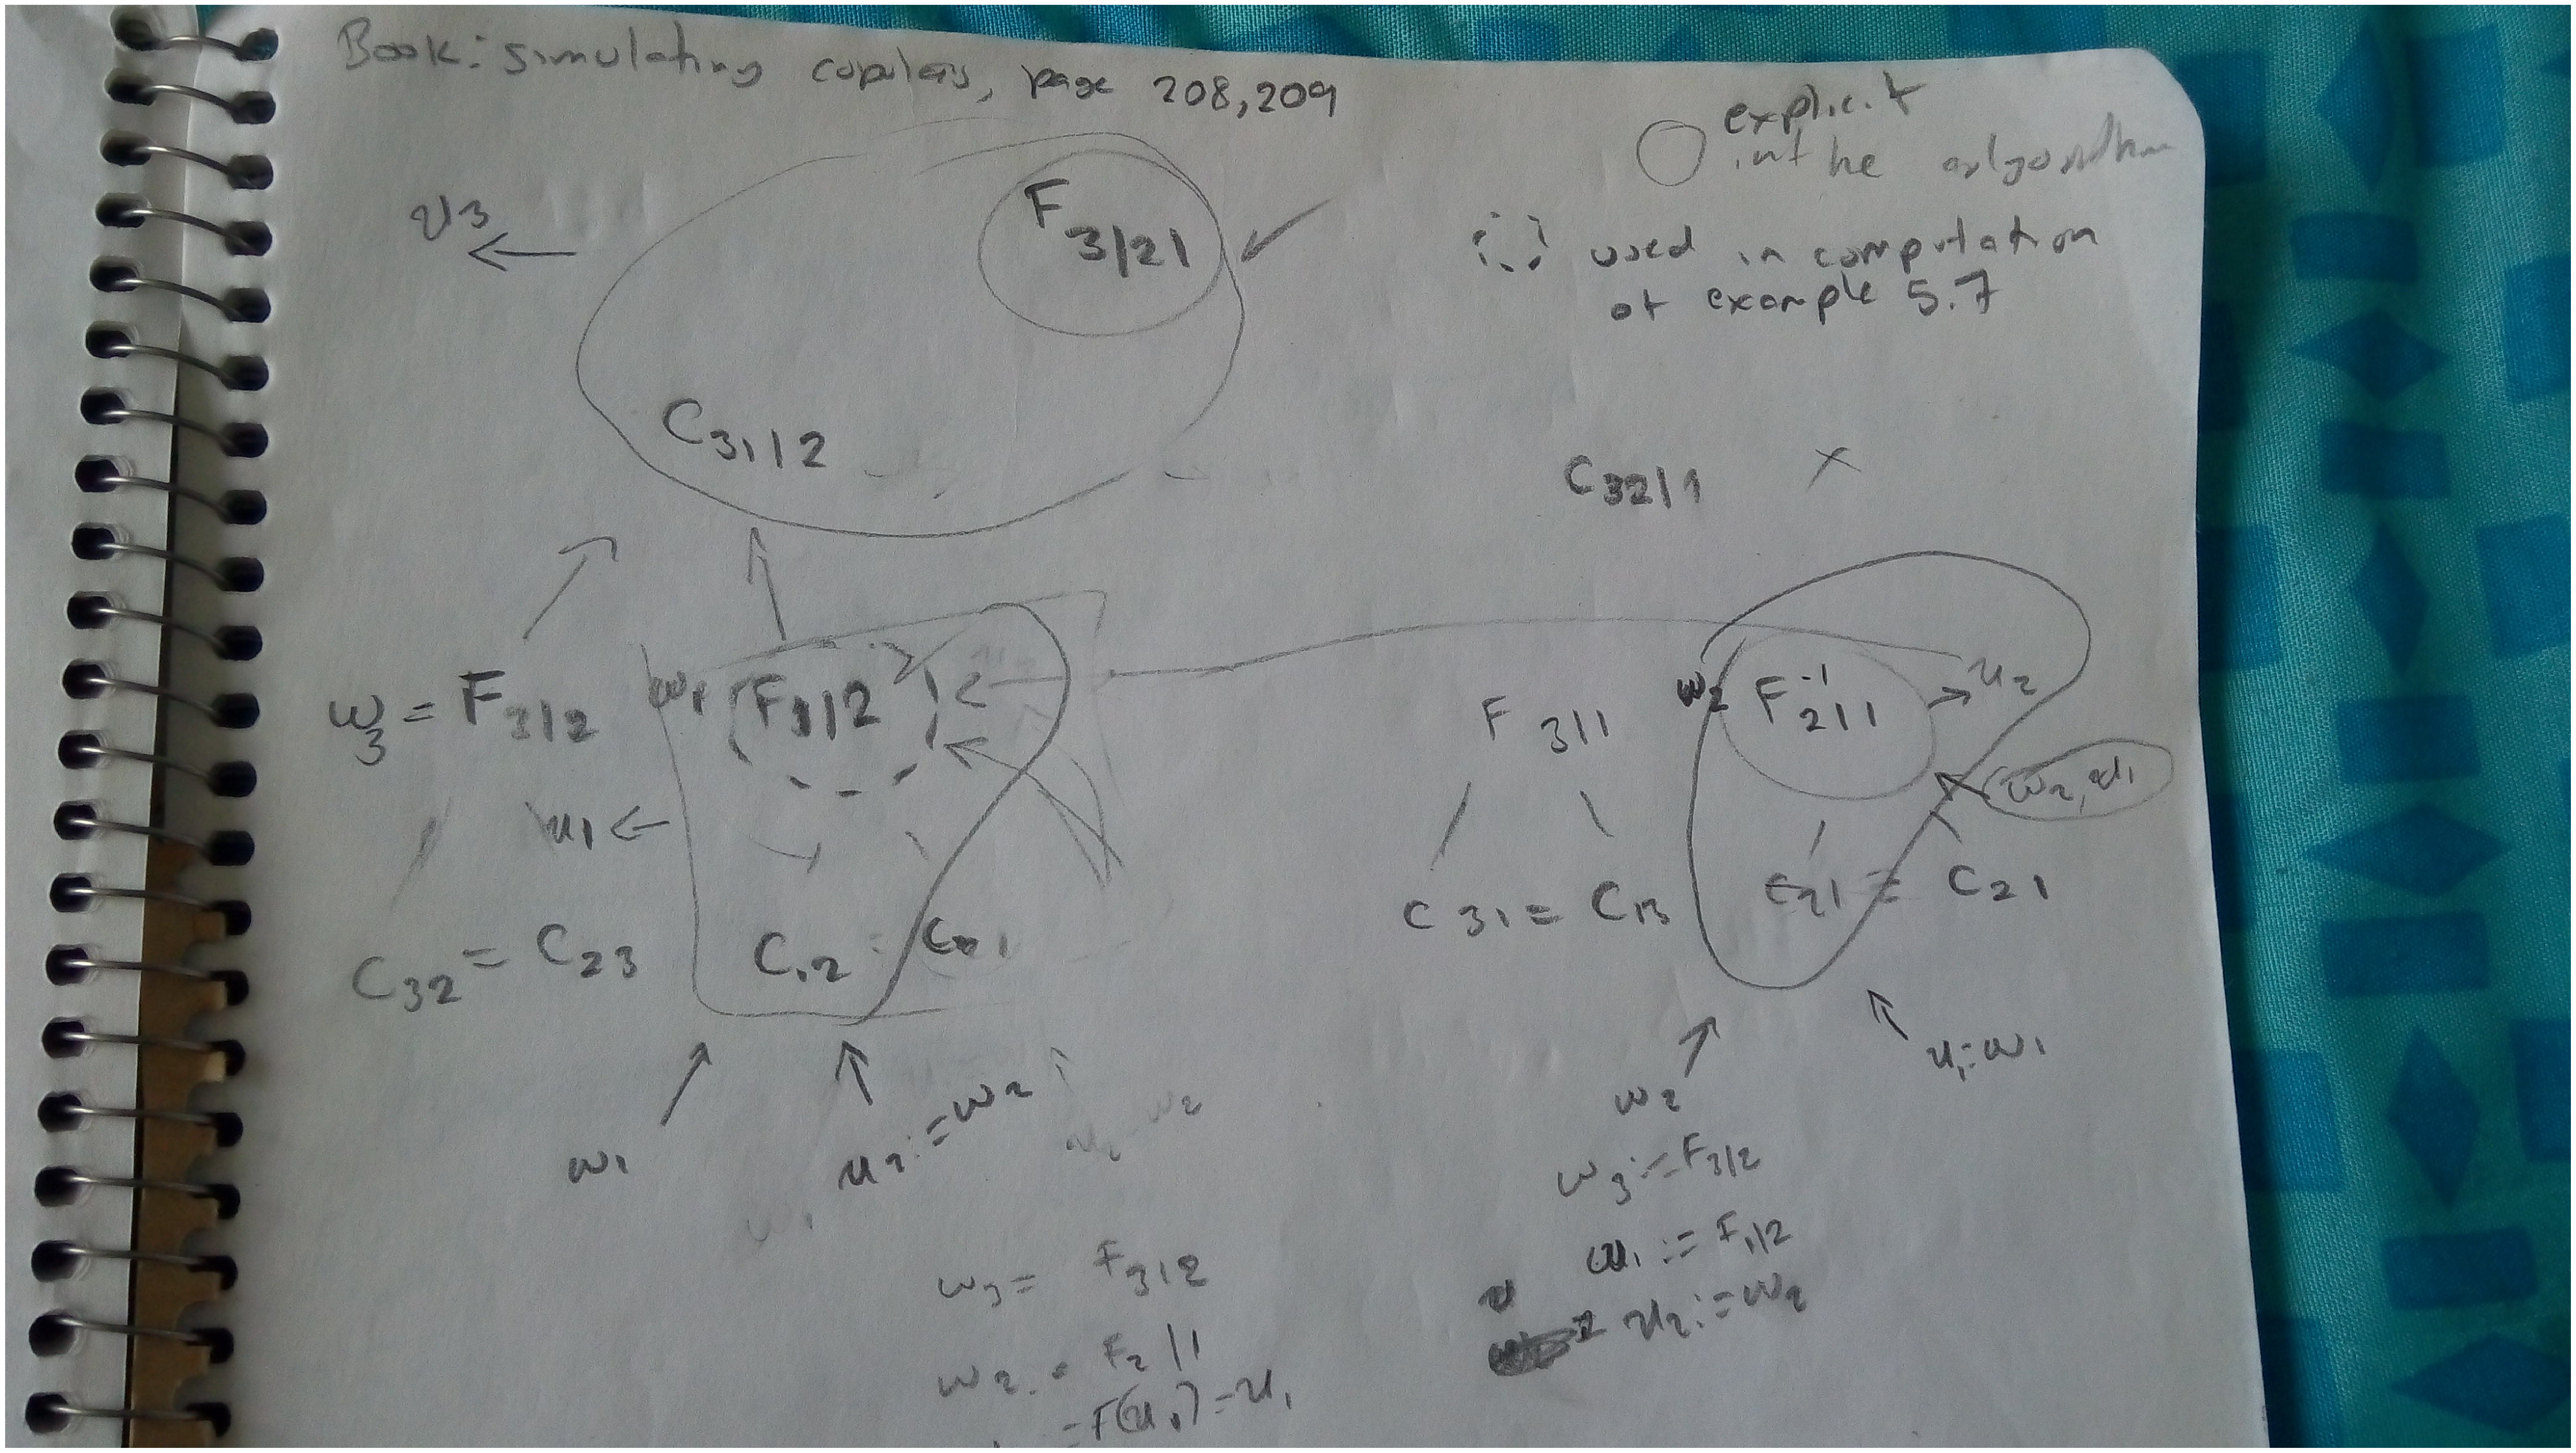
\includegraphics[width=0.9\textwidth]{SimTree}

\section{C\'{o}pulas de Bernstein: caso general multivariado}
 
%Una de las bases para aproximar funciones son los polinomios de Bernstein que en el caso univariado tienen la siguiente forma \citep{sancetta_bernstein_2004}: 
%\begin{equation}
%P_{v}^{m}(u) = \binom{m}{v} u^{v} (1 - u)^{m-v}
%\label{e:BernPoly1D}
%\end{equation}

%Estas funciones base ya han sido utilizadas dentro de la estad\'istica al aproximar funciones cuantiles \citep{munoz-perez_estimating_1987} y de manera aplicada en la simulaci\'on \citep{hernandez-maldonado_joint_2012,hernandez-maldonado_joint_2012-1,hernandez-maldonado_trivariate_2012,erdely-ruiz_modeling_2011,erdely_nonparametric_2009,diaz2015vine}. Este enfoque es no param\'etrico y se utilizar\'a para modelar las funciones de distribuci\'on marginales en este trabajo.

En el caso multivariado, para modelar dependencias, una aproximaci\'{o}n de una funci\'{o}n $d$-dimensional utilizando los polinomios de Bernstein toma la siguiente forma:

\begin{equation}
	G(u_1, \ldots, u_d) =
	\sum_{v_1 = 0}^{m_1} \dots \sum_{v_d = 0}^{m_d}
	\alpha
	\left(
		\frac{v_1}{m_1}, \ldots, \frac{v_d}{m_d}
	\right)
	\prod_{i = 1}^{d} B(u_i|v_i,m_i)
\label{e:BernPoly}
\end{equation}

Si definimos los arreglos ordenados (vectores) $n$-dimensionales

\begin{align}
	\mathbf{m} & := (m_1, \dots, m_n) \\
	\mathbf{u} & := (u_1, \ldots, u_n) \\
	\mathbf{v} & := (v_1, \ldots, v_n) \\
	\mathbf{0} & := (0, \ldots, 0)
\end{align}

entonces podemos definir

\begin{equation}
	\sum_{\mathbf{v} = \mathbf{0}}^{\mathbf{m}} := 
	\sum_{v_1 = 0}^{m_1} \dots \sum_{v_d = 0}^{m_d}
\end{equation}

y por lo tanto la ecuaci\'on (\ref{e:BernPoly}) se puede expresar como

\begin{equation}
	G(\mathbf{u}) =
	\sum_{\mathbf{v} = \mathbf{0}}^{\mathbf{m}}
	\alpha
	\left(
		\frac{v_1}{m_1}, \ldots, \frac{v_d}{m_d}
	\right)
	\prod_{i = 1}^{d} B(u_i|v_i,m_i)
\end{equation}

El caso m\'as sencillo se obtiene cuando $n=1$:

\begin{equation}
	G(u) = \sum_{v=0}^m
	\alpha
	\left(
		\frac{v}{m}
	\right)
	B(u|v,m)
\end{equation}

Dado que los polinomios satisfacen de manera natural muchas de las propiedades de las funciones de distribuci\'{o}n acumulada, los polinomios de Bernstein han demostrado ser una buena aproximaci\'{o}n de la c\'{o}pula emp\'{i}rica, que en el caso bivariado toma la siguiente forma \citep{deheuvels_fonction_1979}:

Para las simulaciones es importante tener la derivada de (\ref{e:BernPoly}), lo cual se puede obtener haciendo uso de \ref{e:bernCopDer}:  

\begin{align} \label{e:bernCopDer} % Bernstein copula derivative
	\frac{\partial G}{\partial u_l} &=
	\frac{\partial }{\partial u_l}
	\left[
		\sum_{v_1 = 0}^{m_1} \dots \sum_{v_l = 0}^{m_l}
		\dots \sum_{v_d = 0}^{m_d}
		\alpha
		\left(
			\frac{v_1}{m_1}, \ldots,
			\frac{v_l}{m_l}, \ldots,
			\frac{v_d}{m_d}
		\right)
		\prod_{i = 1}^{d} B(u_i|v_i,m_i)
	\right] \\
	&= 
		\sum_{v_1 = 0}^{m_1} \dots \sum_{v_d = 0}^{m_d}
		\prod_{i \ne l} B(u_i|v_i,m_i)
		\frac{\partial }{\partial u_l}
	\left[
		\sum_{v_l = 0}^{m_l}
		\alpha
		\left(
			\frac{v_1}{m_1}, \ldots,
			\frac{v_d}{m_d}
		\right)
		B(u_l|v_l,m_l)
	\right] \\
	&= 
		\sum_{v_1 = 0}^{m_1} \dots \sum_{v_d = 0}^{m_d}
		\prod_{i \ne l} B(u_i|v_i,m_i)
		\frac{\partial }{\partial u_l}
	\left[
		m_l
		\sum_{v_l = 0}^{m_l - 1}
		\Delta_l \alpha
		\left(
			\frac{v_1}{m_1}, \ldots,
			\frac{v_d}{m_d}
		\right)
		B(u_l|v_l,m_l)
	\right] 
\end{align}

El operador $k$-dimensional diferencia finita hacia adelante se define como

\begin{equation}
	\Delta_{1,\ldots,k} \alpha
	\left(
		\frac{v_1}{m}, \ldots, \frac{v_k}{m}
	\right)
	=
	\sum_{l_1=0}^1 \cdots \sum_{l_k = 0}^1
	(-1)^{k+l_1+\cdots+l_k}
	\alpha
	\left(
		\frac{v_1 + l_1}{m}, \ldots, \frac{v_k + l_k}{m}
	\right)
\end{equation}

En el caso univariado $k = 1$:

\begin{align}
	\Delta_1 \alpha
	\left(
		\frac{i}{m}
	\right)
	&= \sum_{l = 0}^1 (-1)^{1 + 1}
	\alpha
	\left(
		\frac{i+l}{m}
	\right) \\
	&=
	\alpha \left( \frac{i + 1}{m} \right) - 
	\alpha \left(\frac{i}{m}      \right)
\end{align}

En el caso multivariado haciendo la diferencia finita de una sola variable:

\begin{align}
	\Delta_r
	\alpha
	\left(
		\frac{i_1}{m}, \cdots,\frac{i_d}{m} 
	\right)
	&= \sum_{l = 0}^1 (-d)^{d + 1}
	\alpha
	\left(
		\frac{i_r+l}{m}
	\right) \\
	&=
	\alpha \left( \frac{i_r + 1}{m} \right) - 
	\alpha \left(\frac{i_r}{m}      \right)
\end{align}

La diferencia finita de la c\'opula emp\'irica bivariada con respecto a la primera variable se reduce a la \autoref{e:forwardDiff2D}.

%La c\'{o}pula de Bernstein se obtiene cuando sustituimos la ecuaci\'{o}n \ref{e:empCop} en la \ref{e:BernPoly}, es decir haciendo $\alpha(\cdot) = C_n(\cdot)$.

\section{C\'opulas multivariadas para vectores aleatorios con componentes orientadas}\label{s:copMvariateDir}

N\'otese que en el trabajo que se ha mostrado hasta ahora sobre datos peri\'odicos solamente se ha hablado de c\'opulas bivariadas. Para el caso \(m\)-variado no se hab\'ia mostrado el modelo de c\'opulas dentro del contexto de las c\'opulas de Bernstein que tome en cuenta cualquier cantidad de variables aleatorias peri\'odicas. La c\'opula densidad \(m\)-variada de Bernstein (Sancetta \& Satchell, 2004, sec. 4.1) es una generalizaci\'on de la ecuaci\'on (9)

$${\hat{c}}_{B}\left( u_{1},\ u_{2},\cdots,\ u_{m} \right)\  = \sum_{j_{1} = \ 1}^{k}{\sum_{j_{2} = \ 1}^{k}\cdots\ \sum_{j_{m} = 1}^{k}p_{j_{1},j_{2},\cdots,j_{m}}\prod_{i\  = \ 1}^{m}{\beta\left( u_{i} \middle| j_{i},k - j_{i} + 1 \right)\ }}$$

Para imponer las condiciones de periodicidad sobre la variable aleatoria \(\mathcal{L}_{1}\)-\'esima, \(\mathcal{L}_{1} \in \left\{ 1,2,\ldots,m \right\}\) se agregan condiciones similares a (16)

$${\tilde{p}}_{j_{1}\cdots 1\cdots j_{m}} = {\tilde{p}}_{j_{1}\cdots k\cdots j_{m}} = \frac{p_{j_{1}\cdots 1\cdots j_{m}} + p_{j_{1}\cdots k\cdots j_{m}}}{2}$$

Para \(j_{i} = 1,\ldots,k\), con
\(i \in \left\{ 1,2,\ldots,\mathcal{L}_{1} - 1,\mathcal{L}_{1} + 1,\ldots,m \right\}\),
i.e., \(i \neq \mathcal{L}_{1}\)

\({\tilde{p}}_{j_{1}\cdots j_{\mathcal{L}_{1}}\cdots j_{m}} = p_{j_{1}\cdots j_{\mathcal{l}_{1}}\cdots j_{m}}\)

Para \(j_{\mathcal{L}_{1}} \neq 1,k\).

Se puede demostrar que la c\'opula converge uniformemente.

Como es de esperarse, la ecuaci\'on (22) se reduce a la ecuaci\'on (16) en el caso bivariado cuando \(\mathcal{L}_{1} = 1\).

N\'otese que si aplicamos nuevamente las ecuaciones (24) a las \(\tilde{p}\), pero esta vez a la variable aleatoria \(\mathcal{L}_{2}\)-\'esima, con \(\mathcal{L}_{1} \neq \mathcal{L}_{2}\), obtenemos el caso de dos variables aleatorias peri\'odicas

\({\tilde{\tilde{p}}}_{j_{1}\cdots j_{\mathcal{L}_{1}}\cdots 1\cdots j_{m}} = {\tilde{\tilde{p}}}_{j_{1}\cdots j_{\mathcal{L}_{1}}\cdots k\cdots j_{m}} = \frac{{\tilde{p}}_{j_{1}\cdots j_{\mathcal{L}_{1}}\cdots 1\cdots j_{m}} + {\tilde{p}}_{j_{1}\cdots j_{\mathcal{L}_{1}}\cdots k\cdots j_{m}}}{2}\)

Para \(j_{i} = 1,\ldots,k\), con
\(i \in \left\{ 1,2,\ldots,\mathcal{L}_{2} - 1,\mathcal{L}_{2} + 1,\ldots,m \right\}\),
i.e., \(i \neq \mathcal{L}_{2}\)

\({\tilde{\tilde{p}}}_{j_{1}\cdots j_{\mathcal{L}_{1}}\cdots j_{\mathcal{L}_{2}}\cdots j_{m}} = {\tilde{p}}_{j_{1}\cdots j_{\mathcal{L}_{1}}\cdots j_{\mathcal{L}_{2}}\cdots j_{m}}\)

Para \(j_{\mathcal{L}_{2}} \neq 1,k\). 

Que para \(j_{\mathcal{L}_{1\ }} = 1,k\) y \(j_{\mathcal{L}_{2}} = 1,k\), es decir, en las esquinas frontera.

\begin{align}
	{\tilde{\tilde{p}}}_{j_{1}\cdots 1\cdots 1\cdots j_{m}} &= 
{\tilde{\tilde{p}}}_{j_{1}\cdots 1\cdots k\cdots j_{m}} = 
{\tilde{\tilde{p}}}_{j_{1}\cdots k\cdots 1\cdots j_{m}} = 
{\tilde{\tilde{p}}}_{j_{1}\cdots k\cdots k\cdots j_{m}} \\
&= \frac{\frac{p_{j_{1}\cdots 1\cdots 1\cdots j_{m}} + p_{j_{1}\cdots k\cdots 1\cdots j_{m}}}{2} + \frac{p_{j_{1}\cdots 1\cdots k\cdots j_{m}} + p_{j_{1}\cdots k\cdots k\cdots j_{m}}}{2}}{2} \\
&= \frac{p_{j_{1}\cdots 1\cdots 1\cdots j_{m}} + p_{j_{1}\cdots k\cdots 1\cdots j_{m}} + p_{j_{1}\cdots 1\cdots k\cdots j_{m}} + p_{j_{1}\cdots k\cdots k\cdots j_{m}}}{2^{2}}
\end{align}


N\'otese que para el caso particular de la c\'opula bivariada la ecuaci\'on (23) se reduce a la ecuaci\'on (20).

De esta manera se podr\'ia continuar con el algoritmo para dar la periodicidad a las variables aleatorias requeridas.

\begin{figure}
	\centering
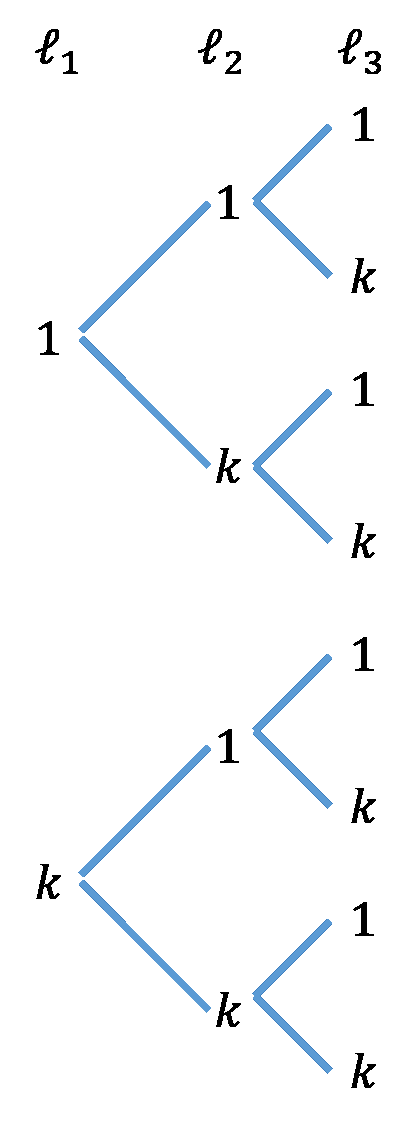
\includegraphics[width=0.95647in,height=2.74852in]{generalBernstein}
	\caption{Diagrama de \'arbol que muestra c\'omo se van agregando la condici\'on de periodicidad a las variables aleatorias para la c\'opula de Bernstein multivariada. Aqu\'i se muestra el caso para 3 variables aleatorias peri\'odicas. N\'otese que tambi\'en muestra la cantidad de sumandos de los elementos de las esquinas, que para este caso es \(2^{3}\).}
	\label{f:treeDiagPer}
\end{figure}


